\documentclass[a4paper, 12pt, oneside]{article}
\usepackage[T1]{fontenc}
\usepackage{aurical}
\usepackage{booktabs}
\usepackage{textalpha}
\usepackage{url}
\setlength{\emergencystretch}{15pt}
\usepackage{fancyhdr}
\usepackage{amssymb}
\usepackage{lscape}
\usepackage{longtable}
\usepackage{tablefootnote}
\usepackage{array}
\usepackage{imakeidx}
\usepackage{float}
\usepackage{qtree}
\usepackage{microtype}
\usepackage{sectsty}
\usepackage[titles]{tocloft}

\allsectionsfont{\Fontauri}
\sectionfont{\Fontauri\Huge}
\subsectionfont{\Fontauri\LARGE}
\subsubsectionfont{\Fontauri\Large}

\usepackage[dvipsnames]{xcolor}
\usepackage{eso-pic,graphicx}
\usepackage[top=70mm, bottom=45mm, outer=29mm, inner=29mm]{geometry}
\setlength{\columnsep}{90pt}

\usepackage{setspace}
\onehalfspacing

\def\arraystretch{1.15}

% change color of text, example replace all \color{Goldenrod} with \color{lightgray}
\definecolor{customColor}{RGB}{102, 2, 60}

\makeatletter % change only the display of \thepage, but not \thepage itself:
\patchcmd{\ps@plain}{\thepage}{\bfseries\large\color{customColor}{\thepage}}{}{}
\makeatother

\color{customColor}

\begin{document}
\Fontauri
\bfseries
\pagestyle{plain} % after changing a pagestyle command, it's necessary to invoke it explicitly

\renewcommand\thefootnote{\Fontauri\bfseries{\tiny\arabic{footnote}}}
\let\oldfootnote\footnote
    \renewcommand{\footnote}[1]{\oldfootnote{\Fontauri\bfseries\large#1}}

\AddToShipoutPictureBG{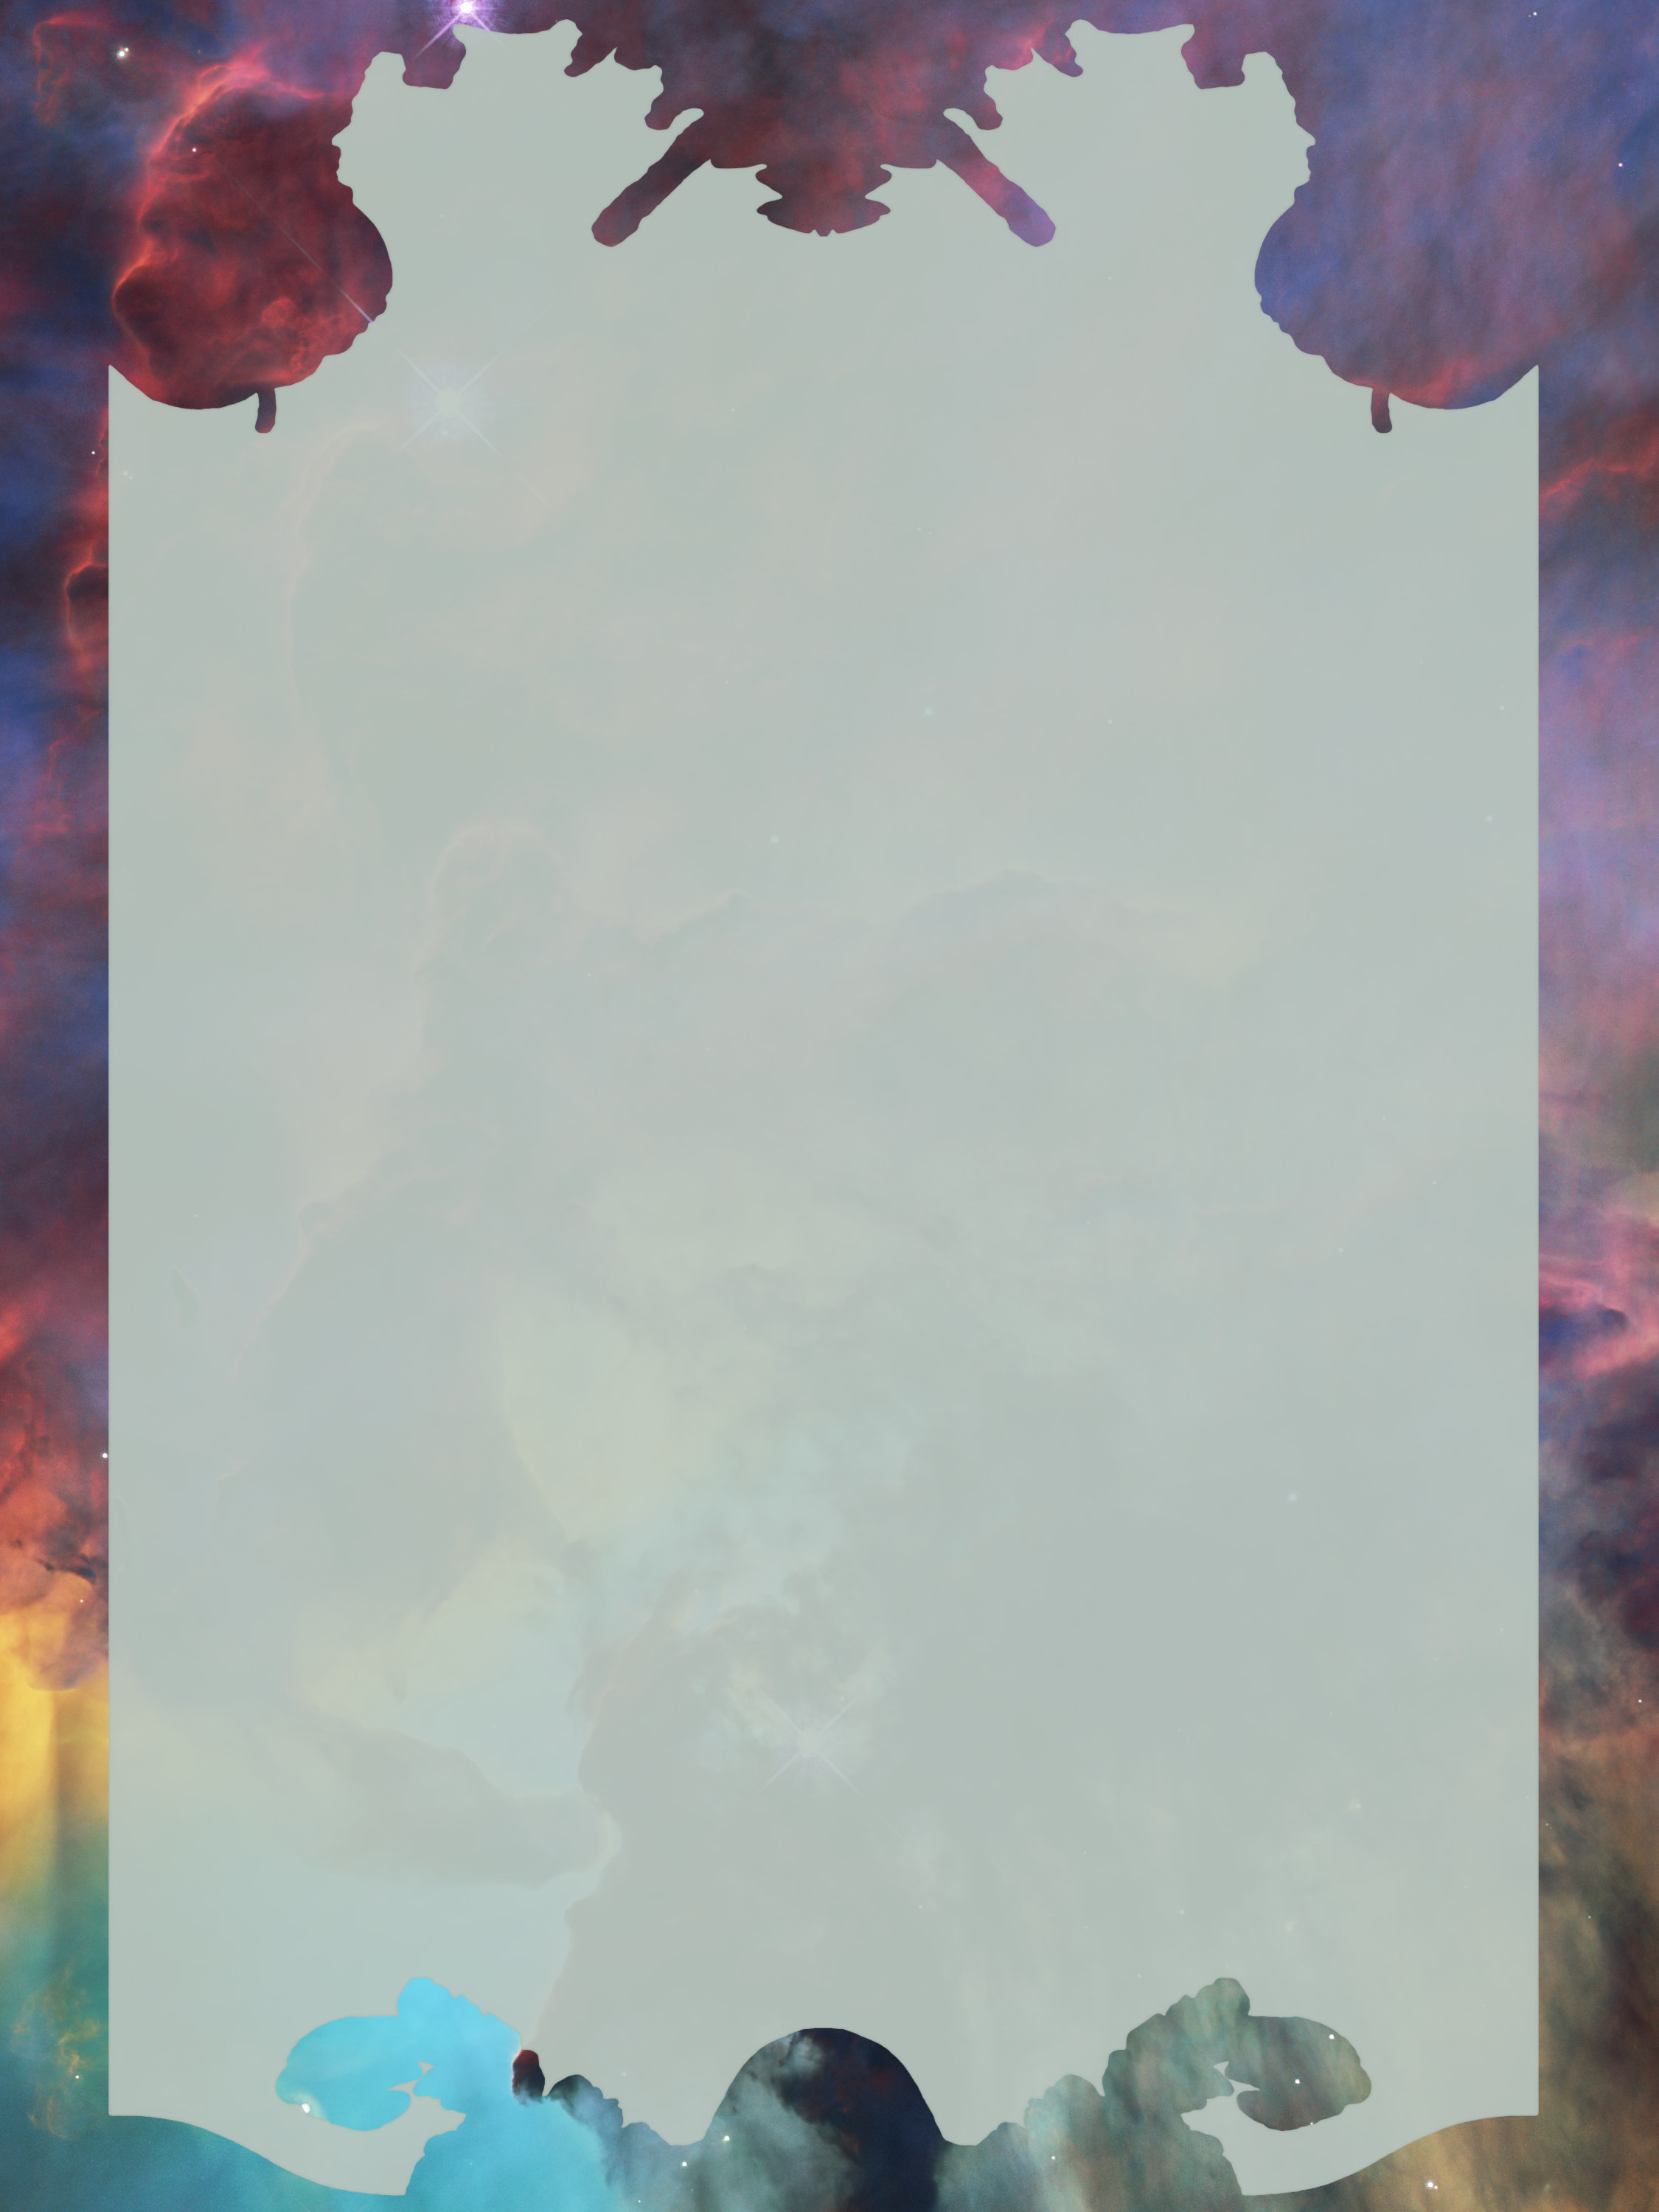
\includegraphics[width=\paperwidth,height=\paperheight]{hubble.jpeg}}

\renewcommand{\contentsname}{
\Fontauri{Index}
}
\renewcommand{\listfigurename}{
\Fontauri{List of Figures}
}

\renewcommand{\cftsecfont}{\Fontauri}
\renewcommand{\cftsubsecfont}{\Fontauri}
\renewcommand{\cftsubsubsecfont}{\Fontauri}

% fix toc page numbers
\let\origcftsecfont\cft
\let\origcftsecpagefont\cftsecpagefont
\let\origcftsecafterpnum\cftsecafterpnum
\renewcommand{\cftsecpagefont}{\Fontauri{\origcftsecpagefont}}
\renewcommand{\cftsecafterpnum}{\Fontauri{\origcftsecafterpnum}}
\let\origcftsubsecpagefont\cftsubsecpagefont
\let\origcftsubsecafterpnum\cftsubsecafterpnum
\renewcommand{\cftsubsecpagefont}{\Fontauri{\origcftsubsecpagefont}}
\renewcommand{\cftsubsecafterpnum}{\Fontauri{\origcftsubsecafterpnum}}
\let\origcftsubsubsecpagefont\cftsubsubsecpagefont
\let\origcftsubsubsecafterpnum\cftsubsubsecafterpnum
\renewcommand{\cftsubsubsecpagefont}{\Fontauri{\origcftsubsubsecpagefont}}
\renewcommand{\cftsubsubsecafterpnum}{\Fontauri{\origcftsubsubsecafterpnum}}

\begin{titlepage} % Suppresses headers and footers on the title page
	\centering % Centre everything on the title page
	\scshape % Use small caps for all text on the title page

	%------------------------------------------------
	%	Title
	%------------------------------------------------
	
	\rule{\textwidth}{1.6pt}\vspace*{-\baselineskip}\vspace*{2pt} % Thick horizontal rule
	\rule{\textwidth}{0.4pt} % Thin horizontal rule
	
	\vspace{0.75\baselineskip} % Whitespace above the title

        {\Huge An Essay \\ on Meteorites \\} % Title
	
	\vspace{0.75\baselineskip} % Whitespace below the title
	
	\rule{\textwidth}{0.4pt}\vspace*{-\baselineskip}\vspace{3.2pt} % Thin horizontal rule
	\rule{\textwidth}{1.6pt} % Thick horizontal rule
	
	\vspace{1\baselineskip} % Whitespace after the title block
	
	%------------------------------------------------
	%	Subtitle
	%------------------------------------------------
	
	{By \scshape\Large R. P. Greg, FGS \\} % Subtitle or further description
	
	\vspace*{1\baselineskip} % Whitespace under the subtitle
	
	%------------------------------------------------
	%	Editor(s)
	%------------------------------------------------

	\vspace{1\baselineskip} % Whitespace before the editors

    %------------------------------------------------
	%	Cover photo
	%------------------------------------------------
	
	%\includegraphics[scale=1]{cover}
	
	%------------------------------------------------
	%	Publisher
	%------------------------------------------------
		
	\vspace*{\fill}% Whitespace under the publisher logo
	
	November, 1855.% Publication year
	
	\vspace{1\baselineskip} % Whitespace under the publisher logo

        Internet Archive Online Edition  % Publication year
	
	{\small Attribution NonCommercial ShareAlike 4.0 International } % Publisher
\end{titlepage}
\setlength{\parskip}{1mm plus1mm minus1mm}
\setcounter{tocdepth}{3}
\setcounter{secnumdepth}{3}
\pagestyle{fancy}
\fancyhf{}
\cfoot{\Fontauri{\thepage}}
\tableofcontents
\clearpage
\Large
\section*{Preface.}
\paragraph{}
The following Essay originally appeared in the Philosophical Magazine for November and December 1854. I have been induced to publish it in a separate form. It has undergone both revision and addition; and the \emph{lunar} theory of the origin of meteorites has been noticed at some length.

The Catalogue and Tables have been constructed at considerable trouble; and as being by far the most complete yet published, may be found useful to those who collect, or take any interest in those bodies.

Through the nature and characteristics of this class of phaenomena are much better understood than formerly, the theoretical and cosmical part is still open to discussion.

\bigskip

R. P. G.

\bigskip

Manchester, November 1855.
\clearpage
\section{Observations on Meteorolites or Aërolites, considered Geographically, Statistically, and Cosmically.}
\paragraph{}
It is many years since any attempt has been made to give a complete list of well-authenticated meteoric falls; recently, indeed, M. Partsch of Vienna has published an interesting account, as well as catalogue, of the meteoric irons and stones in the Imperial Museum of that city; and Professor Shepard of the United States has also given us a list of the meteorites in his own collection, as well as a \emph{thesis} on American meteorites; but I am ignorant of anything approaching a complete or compendious catalogue of the falls of these bodies.

The accompanying catalogue has been carefully compiled from various sources\footnote{\Fontauri{Such as old volumes of the Philosophical Transactions; the Philosophical Magazine; Brewster's Encyclopaedia, article ``Meteorite''; Partsch's, Shepard's and Chladni's Catalogues; the volumes of the British Association; Silliman's Journal; \emph{Comptes Rendus; Annales de Chimie et de Physique}, vol. 31.; Nicholson's Journal of Philosophy; Professor Clark's Thesis on Iron Meteoric Masses; and sundry other periodicals, both scientific and literary.}}; where possible, concise particulars, not only as to date and locality, are given, but mention is also made of weights, specific gravity, appearances, etc.; and several analytical and statistical tables are added, which may not be without importance in the present as well as future consideration of this subject.

Great care has been taken to avoid erroneous dates or confusion of localities; and queries are occasionally annexed, where there wants evidence to establish fully the authenticity or correctness of the fall.

It is more especially my present object to investigate some of the results apparently indicated by these tables, constructed purposely from the general catalogue; and I shall consider the subject, first \emph{geographically}, \emph{i. e.} with regard to the \emph{geographical} distribution or deposition of aërolites on the surface of the globe; secondly, \emph{statistically}, with reference to dates and numbers; and thirdly, if I may use the term, \emph{cosmically}.

Considerable allowance must be made in the following, as indeed in all considerations respecting these singular bodies; but I am of opinion that the number of falls now brought together in a tabulated form will be sufficient to furnish us with some evidence, if indeed only of a negative kind, to start from. The three following tables would indicate a pretty equable occurrence of meteoric falls on the surface of our earth, a point by no means without importance. Due allowance must of course be made for various counteracting influences, such as preponderance of sea and uninhabited countries in certain latitudes, and want of historical or scientific records among particular nations, etc.
\subsection{Table A.}
\begin{table}[H]
    \centering
    \bfseries
    \Fontauri
    \footnotesize
    \begin{tabular}{|p{40mm}|l|l|l|p{17mm}|}
    \hline
         Countries. & Stones. & Irons. & Total. & Average latitude. $^\circ$ \\ \hline
        France & 34 & 1 & 35 & 46 N. \\ \hline
        Ireland and Great Britain & 20 & 1 & 21 & 53 N. \\ \hline
        Bavaria, Prussia; Germany & 38 & 6 & 44 & 51 N. \\ \hline
        Hungary, Bohemia; Austria & 28 & 5 & 33 & 48 N. \\ \hline
        Switzerland & 2 & ~ & 2 & 46 N. \\ \hline
        Lombardy, Piedmont, Sicily; Italy & 33 & 1 & 34 & 43 N. \\ \hline
        Portugal and Spain & 9 & ~ & 9 & 40 N. \\ \hline
        European Russia & 14 & 1 & 15 & 54 N. \\ \hline
        Finland and Siberia & 4 & 3 & 7 & 63 N. \\ \hline
        Sweden & 1 & ~ & 1 & 60 N. \\ \hline
        Asia Minor, Crete; Turkey & 10 & 1 & 11 & 40 N. \\ \hline
        Egypt, Arabia and N. Africa & 6 & 1 & 7 & 30 N. \\ \hline
        Tartary, Persia and Central Asia & 1 & 2 & 3 & 35 N. \\ \hline
        Japan and China & 23 & ~ & 23 & 18 N. \\ \hline
        Ceylon and India & 19 & 3 & 22 & 20 N. \\ \hline
        United States & 18 & 36 & 54 & 35 N. \\ \hline
        Greenland & 1 & 2 & 3 & 65 N. \\ \hline
        West Indies and Mexico & 2 & 10 & 12 & 25 N. \\ \hline
        Sandwich Islands & 1 & ~ & 1 & 20 N. \\ \hline
        South Africa & 2 & 2 & 4 & 30 S. \\ \hline
        Java & 1 & ~ & 1 & 10 S. \\ \hline
        South America & 1 & 8 & 9 & 20 S. \\ \hline
        Canada & ~ & 1 & 1 & ~ \\ \hline \hline
        Totals & 268 & 84 & 352 & ~ \\ \hline
    \end{tabular}
\end{table}
\subsection{Table B. --- Showing the number of Meteoric Depositions recorded, arranged according to zones of Latitude, North.}
\begin{table}[H]
    \centering
    \bfseries
    \Fontauri
    \begin{tabular}{|l|r|}
    \hline
        Between N. Latitude 5$^\circ$ and 10$^\circ$ & 3 \\ \hline
        Between N. Latitude 10$^\circ$ and 20$^\circ$ & 18 \\ \hline
        Between N. Latitude 20$^\circ$ and 30$^\circ$ & 35 \\ \hline
        Between N. Latitude 30$^\circ$ and 40$^\circ$ & 75 \\ \hline
        Between N. Latitude 40$^\circ$ and 50$^\circ$ & 129 \\ \hline
        Between N. Latitude 50$^\circ$ and 60$^\circ$ & 68 \\ \hline
        Between N. Latitude 60$^\circ$ and 70$^\circ$ & 9 \\ \hline \hline
        ~ & 337 \\ \hline
    \end{tabular}
\end{table}
\subsection{Table C. --- Showing the proportion of falls, for several countries, that might be supposed to occur, making due allowance for the relative extent and population of each, taking France as the standard or unit of comparison, and commencing with the year 1790.}
\begin{table}[!ht]
    \centering
    \bfseries
    \Fontauri
    \begin{tabular}{|l|l|l|}
    \hline
         ~ & Actual number. & Computed number. \\ \hline
        France & 19 & 19 \\ \hline
        Great Britain and Ireland & 11 & 12 \\ \hline
        Spain & 5 & 9 \\ \hline
        Germany & 12 & 13 \\ \hline
        Austria & 14 & 13 \\ \hline
        Italy & 11 & 14 \\ \hline
        European Russia & 12 & 31 \\ \hline
        United States & 18 & 8 \\ \hline
    \end{tabular}
\end{table}                
\paragraph{}
The number of meteoric falls recorded for Great Britain, France, Germany, Austria and Italy, is thus shown to have been sixty-seven, in a period of sixty-four years. Taking the area of these five countries at 900,000 square miles, and that of the earth's surface at 197 millions, we obtain 220 as the number of annual falls likely, in the ordmary course of events, to be observed, were the whole surface of our globe peopled with an European density of population and a similar degree of civilization.

Taking, however, into consideration that one-half of mankind is alternately experiencing the darkness of night, when they are not so likely to observe the descent of these bodies or mark the exact spot where they reach the earth's surface, we may fairly, instead of 220, assume 400 as more nearly the number of falls likely to occur under the above-named conditions. What proportion 400 may bear to the entire number that fall, it is not easy to conjecture, though after mature consideration, I am inclined to think that number will exceed one-third of the whole.\footnote{\Fontauri{See Table H., and Note \emph{a}, p. 29.}} It is desirable to bear in mind the probability of a not \emph{unequal} distribution of meteorite falls on the surface of the earth, because it might appear from a too superficial or limited examination, that such was not the case, a view, indeed, apparently adopted by Professor Shepard, in some remarks he published in 1850, respecting the ``Geographical Distribution'' of these bodies. He considers that there are some regions of the earth's surface, or certain zones, towards or in which there is a tendency to ``concentration in the deposition'' of meteoric matter; and he instances particular countries, as Canada, Portugal, Spain, South Italy, Sicily, Hungary, Denmark, Sweden, Norway, and Northern Russia, which furnish few or no instances of meteoric deposition. As regards Norway only can his remarks strictly hold good, as will be admitted on a perusal of the localities given in the catalogue accompanying this paper: that there are some irregularities no one wul deny, yet considering the strange nature of, and the pheanomena exhibited by, these bodies, and making due allowance for various causes likely to affect an observable uniformity of deposition, it is only remarkable how uniformly they have everywhere been observed.\footnote{\Fontauri{For mention of some less important, though not less curious, irregulurities concerning the fall and nature of meteorites, see Note 1. at the end.}}

Professor Shepard correctly takes for the United States the parallel of 37$^\circ$ N. as the line of greatest average meteoric deposition, and for Europe that of 46$^\circ$ N.

A line drawn through the centre of greatest meteoric deposttion in America would, if prolonged so as to include the like centre for Europe, form, with the ordinary parallels of latitude, an angle of about 10$^\circ$ or 11$^\circ$.

I shall now quote Prof. Shepard's own words:---

``If then it appears that these aërial strangers alight upon our earth in such great preponderance over limited areas, can we help admitting that there presides over their descent some great law, or in other words, that these falls take place in accordanee with some fixed plan. The present stage of our knowledge may, indeed, be inadequate to develope what that plan actually is; but when we see so marked an approach, by the courses of our meteoric regions, to the isothermal parallels for the same zones, and again, an observable coincidence between the trends of the meteoric regions and the isodynamic lines, we are strongly tempted to refer the forces of greatest activity concerned in the phaenomenon, to a union of thermal and magnetic action; although it is, at the same time, possible that more powerful local attractions in the surfaces concerned, than exist elsewhere, may also exert some influences over the deposition of these singular bodies.''

I need not say more respecting this part of the subject, except that I must differ from Prof. Shepard, and give my facts and reasons for so doing.

It would indeed be strange should these bodies --- varying in size and weight from half an ounce to 30,000 lbs., sometimes containing no iron at all, and occasionally composed of nothing but iron, having an oblique direction generally from east to west, and a velocity of fifteen to thirty miles in a second, --- be attracted by particular countries more than others, or arrange themselves in zones parallel to the isothermal or isodynamic lines.

The next point I shall draw attention to, are the variations in the number of falls taken in five-yearly periods, from 1795 up to 1854:---
\begin{table}[H]
    \centering
    \bfseries
    \Fontauri
    \begin{tabular}{l r}
         ~ & ~ \\ \hline
        From 1795 to 1800 are described… & 7 \\ \hline
        From 1800 to 1805 are described… & 6 \\ \hline
        From 1805 to 1810 are described… & 13 \\ \hline
        From 1810 to 1815 are described… & 15 \\ \hline
        From 1815 to 1820 are described… & 9 \\ \hline
        From 1820 to 1825 are described… & 12 \\ \hline \hline
        Falls… & 62 \\ \hline \hline
        From 1825 to 1830 are described… & 11 \\ \hline
        From 1830 to 1835 are described… & 7 \\ \hline
        From 1835 to 1840 are described… & 12 \\ \hline
        From 1840 to 1845 are described… & 14 \\ \hline
        From 1845 to 1850 are described… & 11 \\ \hline
        From 1850 to 1854 are described… & 7 \\ \hline \hline
        Falls… & 63 \\ \hline \hline
        Total… & 125 \\ \hline
    \end{tabular}
\end{table}
\paragraph{}
This gives an average of eleven for each of the twelve quinquennial periods, or nearly \emph{two} per annum; but one more fall is recorded for the first moiety of the sixty years than for the second, though one might have expected rather a marked increase during the second period, owing to the increase which has taken place during the last quarter of a century in population and intelligence, as well as facilities for procuring and disseminating information.

Indeed, as but one fall is recorded for each of the years 1852, 1853, 1854 and 1855, and but two for each of the years 1847, 1848, 1849 and 1850, while some years present us with three, four, and even five instances of falls, one is almost led to imagine a temporary if not absolute falling off in the frequency of these phaenomena; whether this may be owing to accident and chance, or to the existence of some unknown cause or cycle, we must, from want of more data, at present remain ignorant.

The following Table, presenting an analysis of the total number of known falls I have been enabled to collect or hear of, arranged according to the falls for each month, from the year AD 1496 to 1855, shows some curious if not indeed important results.
\subsection{Table D.}
 \begin{table}[H]
    \centering
    \bfseries
    \Fontauri
    \begin{tabular}{|l|r|}
    \hline
        Month. & No. \\ \hline
        January & 10 \\
        February & 15 \\
        March & 17 \\
        April & 14.5 \\
        May & 17 \\
        June & 18 \\ \hline
        First half-yearly total & 91.5 \\ \hline
        July & 19.5 \\
        August & 15 \\
        September & 16 \\
        October & 14 \\
        November & 16 \\
        December & 9 \\ \hline
        Second half-yearly total & 89.5 \\ \hline \hline
        N. B. Average & 15.0 \\ \hline
    \end{tabular}
\end{table}
\paragraph{}
It is rather singular how nearly equal the number is for each half-yearly period; but the most important thing to notice is the great falling off for the months of December and January, and the almost corresponding increase for June and July; the two former together only show 19, while the two latter 37.5, or about double.\footnote{\Fontauri{Monsieur Marcel de Serres, in the \emph{Annales de Chimie et de Physique}, vol. 85. p. 262, remarks, that out of sixty-five falls, two-thirds were in June, July and August.}}

It may be argued, that this is in consequence of the days being longer in summer than in winter. While, however, there is but 16 per cent. more daylight in November than in December, the falls of meteorites are, it is seen, more than 50 per cent. more, and while there are ten falls recorded in January, there are fifteen in February, and seventeen in March, months when the days are still nearly as short. November shows considerably more also than December. The difference existing between different countries, in latitude and longitude, will also tend rather to equalize the difference that occurs in the duration or simultaneous commencement of night at any particular period of the year. The ten falls for January are spread over, be it observed, a very long period. There appear only to be four instances in the last hundred years. (See Note 2.)

There is doubtless then some other and more important reason required to account for this marked decrease in the number of aërolites observed in December and January, as well perhaps as for the larger number of falls which have occurred in June and July.

Let it be borne in mind that the earth in her orbit at those periods of the year, is on the sides of the winter and summer solstices respectively, \emph{i. e.} in \emph{perihelion} and \emph{aphelion}.

I shall revert to this part of the subject, and now proceed to the consideration of the following Table which I have constructed, rather roughly indeed, from the reports of Professor Powell, drawn up for, and published by the British Association, in the volumes of its Transactions for the years 1848 to 1853. At best these results can only be relative and approximative.

Column A. denotes the total number of luminous meteors described (or recorded and particularized) in the above-named reports; and column B. the number only of the most remarkable ones.\footnote{\Fontauri{Such as those having a larger \emph{apparent} size than the planet Jupiter, those accompanied by audible explosion, or such as are described as having approached particularly near the surface of the earth.}}
\subsection{Table E. --- Luminous Meteors.}
\begin{table}[H]
    \centering
    \bfseries
    \Fontauri
    \begin{tabular}{|l|l|l|r|}
    \hline
         Months. & A. & B. & Percentage of large ones. \\ \hline
        January & 190 & 13 & 6.8 \\ \hline
        February & 102 & 18 & 18.0 \\ \hline
        March & 117 & 7 & 6.0 \\ \hline
        April & 236 & 15 & 6.7 \\ \hline
        May & 41 & 8 & 20.0 \\ \hline
        June & 88 & 12 & 13.6 \\ \hline
        July & 364 & 20 & 5.5 \\ \hline
        August & 4370 & 25 & 0.6 \\ \hline
        September & 315 & 25 & 7.9 \\ \hline
        October & 320 & 12 & 3.9 \\ \hline
        November & 1470 & 24 & 1.7 \\ \hline
        December & 310 & 19 & 6.1 \\ \hline
    \end{tabular}
\end{table}
\paragraph{}
On comparing this table with Table D, one is struck with several comparative dissimilarities of result. The marked poverty of meteors observed in March, May and June, does not agree with the number of aërolites observed for the same months, as given in Table D, where March and May have over the average number, for the whole year.

In Table E, December has nearly as many as July, September and October; and more than January, February, March, April, May and June. This may perhaps be the result of chance, but not so when we take the months of August and November (Table E.); these two months show a decided and even enormous preponderance in the number of luminous meteors observed, owing principally to the periodic displays which usually take place from the 9th to the 13th of each month.

Referring now to Table D, it will be observed that the number of meteoric stones or aërolites ascertained to have fallen for these two months, does not exceed the average of the whole twelve months.

This deserves some attention, since out of more than 150 meteorites (or aërolites) whose precise date of fall are well ascertained, there are but \emph{four} (see Table F.) which fell on any of the twelve days included between the 9th to 14th days of August and November respectively. From this we are, I think, justified in drawing the conclusion, that, with many phaenomena in common, there does exist a distinetion between meteoric stones or \emph{aërolites} and \emph{luminous meteors}.\footnote{\Fontauri{Prof. D. Olmsted, in an article on the subject of meteors, in the 26th volume of the American Journal of Science, p. 132, 18 strongly of opinion that there is a difference in the nature and origin of aërolites and shooting stars.}} This distinction one may suppose to be somewhat of the same character as that existing between planet and comet; the \emph{former} composed of matter in a solid form and revolving round the sun in orbits less elliptical than the \emph{latter}, but more so than those of the larger planets, the \emph{latter} having also a gaseous or perhaps fluid nature.

Some attempts have been made to ascertain the orbits of the periodically recurring meteor showers of August and November, and Professor Olmsted calculated that the one seen on the night of the 13th of November 1833, had its \emph{aphelion} near the earth's orbit, and its \emph{perihelion} within the orbit of Mercury; that is, its mean distance from the sun lies \emph{within} the earth's orbit. (See Note 3.)

An examination of Table F. is favourable to the idea that there may be \emph{periodic} epochs for aërolites as well as for luminous meteors. This, if true, would certainly be a new and important step gained towards a just consideration of these bodies, and determines for them a place in our solar system.

I have just expressed the opinion that there exists a difference betwcen aërolites and luminous meteors or meteoric showers, and based that opinion partly on the fact that there is no increase in the number of aërolites or meteoric stones which have fallen to the earth at those periods \emph{most} remarkable as epochs for luminous meteors; and on comparing the aërolite epochs (see notes \emph{a} and \emph{b}, Table F.) with those for luminous meteors, this opinion is still further borne out. There is, however, distinctly one exception, and that is November 27-29, an epoch apparently common to both classes alike. It remains, however, to be seen if their periods as well as epochs agree, and whether those years in which the aërolites fall are also unusually rich in meteors. (See Note 4.)

If we connect aërolites with the system of the asteroids, allowing that the earth, at the period of \emph{aphelion} or greatest distance from the sun, is most liable to come near or in contact with them, we must also consider them, like the asteroids, as having a greater mean distance than the earth from the sun, \emph{i. e.} as lying principally \emph{without} the earth's orbit.

I am not now proposing any new theory, but only supporting and carrying out the supposition long ago entertained by Dr. Chladni, and since then advocated by most astronomers, that meteoric stones are \emph{true}, though minute, planetary fragments; but from want of data, no serious attempt at anything amounting to demonstrative proof has yet been made; and there are now many scientific men who attribute to them an atmospheric or lunar origin.\footnote{\Fontauri{See page 16.}} When, therefore, there is still so much conjecture and so much confusion respecting the nature, origin and phaenomena of these bodies, any ray of light is acceptable to the theorist, and anything like fact or tabulated statistics, of value. In continuation, then, and in search of further evidence, this part of our subject may also be incidentally considered in another way.

The average specific gravity of about seventy stones\footnote{\Fontauri{Iron falls are comparatively very rare, as compared with stone falls.}} I find to be 3.4, the highest being about 3.95 and the lowest 1.7; but as those possessing the smallest specific gravity are necessarily the most destructible and fragile, and after meteoric explosion less likely to arrive on the surface of the earth in an entire or tangible state, we may very fairly take their average density nearer the mean of these two extremes, say 3.0.

We may now construct a Table of densities (taking water as 1), which is not without interest, as perhaps bearing on the subject in hand.
\begin{table}[H]
    \centering
    \bfseries
    \Fontauri
    \begin{tabular}{l r r}
    \hline
         ~ & Smyth. & Pierce. \\ \hline
        The density of Mercury is about… & 15.7 & 20.1 \\ \hline
        The density of Venus is about… & 5.9 & 5.1 \\ \hline
        The density of Earth is about… & 5.7 & 5.6 \\ \hline
        The density of Moon is about… & ~ & 3.6 \\ \hline
        The density of Mars is about… & 5.3 & 3.8 \\ \hline
        The density of Aërolites is about… & 3.0 & 3.4 \\ \hline
        The density of Asteroids is about… & ? & ~ \\ \hline
        The density of Jupiter is about… & 1.4 & 2.1 \\ \hline
        The density of Saturn is about… & ~ & 0.76 \\ \hline
    \end{tabular}
\end{table}     
\paragraph{}
There is here some additional evidence that aërolites or meteorites may belong to the series of planets having orbits at a greater mean distance than that of the earth's from the sun. Bearing this in mind, as also the probability of the fact of our meeting with more of them on the side of the summer solstice, or when the earth is at her \emph{aphelion}, I would draw attention to the following extract from a paper in the American Journal of Science for July 1854, entitled ``Considerations on the group of small Planets situated between Mars and Jupiter,'' by M. U. J. Le Verrier; the paper in question being a translation and abbreviation of the original in the \emph{Comptes Rendus}, vol. 37. p. 793:---

``If the perihelia of the asteroids, known and unknown, were distributed uniformly in all parts of the zodiac, the second term of the motion of the pershehon of Mars or of the earth might be neglected; because the action of those masses whose perihelia are situated in one half of the heavens, would be destroyed in this second term by the action of those masses whose perihelia are in the other half. But we have seen that there is great liability to error in reckoning upon such a uniformity in their distribution; the perihelia of twenty out of twenty-six being placed in one half of the heavens, a result doubtless not of chance, and seeming to indicate that the matter \emph{whose mass we are investigating is nearer the sun on the side of the summer solstice than of the winter}. This circumstance must be taken into consideration, not for the purpose of introducing it as an essential condition into the solution of the problem, but, on the contrary, of arriving at a result which shall be independent of it.''

``This consideration will lead us not to make use of the motion of the earth's perihelion, although it is better known than that of Mars. The earth's perihelion being in fact situated in that very portion of the heavens occupied by the perihelia of more than three-fourths of the asteroids, the second term which enters into the expression of its motion may become appreciable as compared with the first and of the contrary sign; inasmuch as these terms are respectively proportional to the excentricities of the terrestrial orbit and the orbits of the small planets, and as the excentricities of these last are at the mean \emph{nine} times greater than that of the earth.''

``The perihelion of Mars is situated much more favourably in relation to the mean direction of the perihelia of the asteroids; and, besides, the excentricity of its orbit is greater. As a result of these two conditions united, the second term which enters into the expression of the motion of the perihelion is only \emph{one-fourth} of the first. Now this superiority of the first term may be expected to continue after the discovery of a great number of new asteroids, \emph{whether this predominance of the perihelia in the mean direction of the summer solstice shall be confirmed, as it probably will be}, or whether we shall be obliged to return to the idea of a uniform distribution of them through every part of the heavens.''

``In accordance with these remarks, I have found that if the mass of the whole group of asteroids was equal to the mass of the earth, it would produce in the heliocentric longitude of the perihelion of Mars an inequality which in a century will amount to eleven seconds. Such an inequality, supposing it to exist, surely could not have escaped the notice of astronomers. If we reflect that this inequality will become strikingly sensible at the moment of the opposition of Mars, we must believe that at present, and although the orbit of Mars has not been determined with perfect accuracy, it cannot nevertheless admit of an error in longitude greater than one-fourth of the inequality which we have pointed out. Hence we conclude that \emph{the sum total of the matter constituting the small planets situated between the mean distances 2.20 and 3.16 cannot exceed about one-fourth of the mass of the earth}.''

In a second memoir (\emph{Comptes Rendus}, t. 37. p. 965) M. Le Verrier establishes the following propositions:---
\begin{enumerate}
    \item ``The excentricities of the orbits of the known asteroids can suffer very small changes as the effect of perturbation. These excentricities, which are now quite large, have then always been and will always remain large.''
    \item ``The same is true of the inclination of their orbits; so that the amount of excentricity and inclination answers to the primitive conditions of the formation of the group.''
    \item ``These propositions are only true for distances from the sun above 2.00. An asteroid situated between Mars and the distance of about 2.00 would not be \emph{stable} in the meaning which is attached to that word in celestial mechanics.''
\end{enumerate}
\paragraph{}
\emph{Flora}, which is nearest to the sun of the known asteroids, is 2.20 distant. M. Le Verrier also observes that it is remarkable that a planet has been found almost up to the line which theory assigns as the limit of stability, and that none have been found beyond it. Must we believe that the same cause which has given origin to so many asteroids above the distance 2.00, \emph{has also distributed them below this distance}? but that the excentricities and inclinations of these last being considerably increased, it is at present difficult to discover them, especially because towards their perihelion they will be immersed in the light of the sun, and that coming to their opposition only in their aphelia, they then will be too far from us?
\begin{enumerate}
    \item[4.] ``Owing to the magnitude of their excentricities and their inclinations and the smallness of their variations, the mean motions of the perihelia and of the nodes are proportional to the times.''
\end{enumerate}
\paragraph{}
From the above extracts, if would appear, according to Le Verrier, that there is a probable predominance of the perihelia of the asteroids in the mean direction of our summer solstice; a circumstance, if true, in favour of the opinion I have expressed, that the increase observable in the number of falls recorded for the months of June and July is not quite the result of chance. What Le Verrier says also respecting the probability of undiscovered asteroids outlying as it were the mean limit of stability, argued inductively, is also interesting, and indirectly bears on the point we have been considering. The extreme degree of ellipticity assigned also to the orbits of the asteroids should be noticed.

Proceeding still further in our investigations of this part of the subject, I shall beg leave to make the following quotation from `Smyth's Celestial Cycle,' p. 159. vol. 1., on the subject of the asteroids:---

``Borrowing from La Place's conjecture before alluded to of a great contraction of the sun's atmosphere, a convulsive disorganization of some planet may be supposed to have taken place, by a force capable of overcoming the mutual attraction of its particles, and the mass of matter so broken would inevitably be dispersed in every direction, and in parts of various sizes.''

``The impulses given by the explosion would gradually diminish, and the parts, in gravitating towards the sun, would become influenced by progression and rotation. To this view there does not appear to be any demonstrable objection. It was suggested that under such a disruption the form of the orbits assumed by the fragments, and their inclination to the ecliptic, or to the orbit of the original planet, would depend upon the size of the fragments, or the weight of their respective masses; \emph{the larger mass would deviate least from the original path, while the smaller fragments being thrown off with greater velocity, will revolve in orbits more excentric and more inclined to the ecliptic}. Now that is precisely what happens. Ceres and Vesta are found to be the largest of the asteroids, and their orbits have nearly the same inclination as some of the old planets; while the orbits of the smaller ones, Juno and Pallas, are inclined to the ecliptic 13$^\circ$ and 34.5$^\circ$ respectively. Lagrange computed the force of explosion necessary to burst a planet, and convert a portion of it into a systematic wanderer. By the process described in the \emph{Connaissance des Tems} for 1814, he arrived at the conclusion, that were a fragment to be impelled with a velocity equal to 121 times that of a cannon-ball, it would become a \emph{direct} comet, but a \emph{retrograde} one if the velocity were 156 times. With weaker impulse, however, the frazment would describe an ellipse, and thus, it is presumed, the asteroids probably were impelled with only twenty times that velocity. The exact circumstances of these extraordinary bodies are not yet sufficiently determined, and the correction of future observations is urgently necessary; but the following Table, constructed from details in the Nautical Almanae for 1845, exhibits a very close approximation to their principal elements. The planets are arranged in their order of distance from the sun, and in the semi-axes of their orbits; the semi-axis of the earth's orbit is taken as unity.''
\begin{table}[!ht]
    \centering
    \footnotesize
    \Fontauri
    \begin{tabular}{|p{20mm}|l|l|l|l|}
    \hline
         Elements. & Vesta. & Juno. & Ceres. & Pallas. \\ \hline
        Mean longitude… & 69$^\circ$ 32$^\prime$ 15.3$^\prime$$^\prime$ & 115$^\circ$ 43$^\prime$ 15.1$^\prime$$^\prime$ & 327$^\circ$ 41$^\prime$ 07.8$^\prime$$^\prime$ & 304$^\circ$ 56$^\prime$ 26.4$^\prime$$^\prime$ \\ \hline
        Longitude of perihelion… & 251$^\circ$ 02$^\prime$ 37.4$^\prime$$^\prime$ & 54$^\circ$ 08$^\prime$ 33.3$^\prime$$^\prime$ & 148$^\circ$ 14$^\prime$ 06.2$^\prime$$^\prime$ & 121$^\circ$ 22$^\prime$ 43.5$^\prime$$^\prime$ \\ \hline
        Longitude of ascending node… & 103$^\circ$ 20$^\prime$ 03.4$^\prime$$^\prime$ & 170$^\circ$ 52$^\prime$ 28.9$^\prime$$^\prime$ & 80$^\circ$ 48$^\prime$ 18.7$^\prime$$^\prime$ & 172$^\circ$ 41$^\prime$ 48.1$^\prime$$^\prime$ \\ \hline
        Inclination to ecliptic… & 7$^\circ$ 08$^\prime$ 23.2$^\prime$$^\prime$ & 13$^\circ$ 03$^\prime$ 05.6$^\prime$$^\prime$ & 10$^\circ$ 37$^\prime$ 08.7$^\prime$$^\prime$ & 34$^\circ$ 37$^\prime$ 40.2$^\prime$$^\prime$ \\ \hline
        Angle of excentricity… & 5$^\circ$ 05$^\prime$ 19.9$^\prime$$^\prime$ & 14$^\circ$ 42$^\prime$ 23.7$^\prime$$^\prime$ & 4$^\circ$ 32$^\prime$ 58.9$^\prime$$^\prime$ & 13$^\circ$ 54$^\prime$ 01.2$^\prime$$^\prime$ \\ \hline
    \end{tabular}
\end{table}
\paragraph{}
``Such are the extraordinary conditions of the asteroids, whose intersecting orbits, leading them almost within hail of each other, so to speak, at the rate of more than 40,000 miles an hour, may eventually lead to mutual disturbances, which the attraction of the larger planets cannot control. Although the strange coincidences attending this group may be \emph{accidental}, in general phrase, yet their phaenomena cannot but be considered as evidence tantamount to demonstration, of their having once composed a single planet, and having diverged by the explosive force of a tremendous cataclysm: and in addition to their orbital vagaries, the bodies themselves are not round, as is said to be indicated by the instantaneous diminution of their light on presenting their \emph{angular} faces.''

There is much here to the point, and confirmatory of the theory and facts I am endeavouring to establish, that meteorites belong to the planetary system, and are perhaps the minute outriders of the group of fragmentary planets called asteroids, or planetoids. It is not improbable that in the course of fifty or one hundred years, supposing due care be used in collecting all information possible regarding the dates and falls of aërolites, and in placing the \emph{data} properly together, that we shall not only readily and certainly determine those epochs, but also the periods in years when the epoch itself again comes round; with such an end in view I have constructed the Table G, but it is not yet sufficiently rich in \emph{data} to admit our arriving at definite results.

Luminous meteors and shooting stars (as well as meteor showers), I would chiefly refer to a class of minute comets, which also no doubt occasionaily, like solid meteorolites, enter the earth's atmosphere and are absorbed, but more frequently pass at a moderate distance.

Anything tending to clear up the confusion that exists in the appearances of the meteor class generally, is of interest and value. Some meteoric appearances are doubtless atmospheric and belong to electric or chemical phaenomena. It has lately been supposed by M. Petit and others, that some may be mere satellites of our own planet revolving with great velocity and at a very moderate distance. Indeed the phaenomena exhibited by these appearances are often so linked together, that one might be ready (too hastily however) to consider them all as one family, the relations of which are not in reality distinguishable from each other.

The Rev. Baden Powell, who has studied this question very attentively, and especially that of luminous meteors, expressed the opinion, at a lecture delivered at the Radcliffe Library, on the 24th June, 1847, that there exists a connexion between aërolites and luminous meteors; and that such small bodies may circulate in the solar system, though probably in small numbers, \emph{unless} truly planetary, or as satellites of some of the larger planets, as of the earth.\footnote{\Fontauri{It has been shown by Walker (see American Philosophical Transactions for 1841), that the influence of the earth's attraction on meteoric bodies approaching near that planet, with planetary velocity, is \emph{not} considerable; at least not equal to any errors of observation in a calculation of their orbits. It has also been proved that the maximum velocity of a meteoric body, revolving as a periodic \emph{satellite of the earth}, cannot exceed 5 /2 [?] miles in a second, whereas the average velocity of these bodies is about fifteen miles per second.}}

M. Arago, in his Popular Lectures on Astronomy, appears to view favourably what is termed the lunar theory, as best adapted to account for the similarity \emph{chemically} existing between meteorites and our own earth.

Dr. Lawrence Smith of Louisville University, U. S., has just published in the American Journal of Science, Second Series, vol. 19. May 1855, an interesting memoir on Meteorites, which deserves attention even from those who may not agree with the theory of their \emph{lunar} origin. He directs attention to the physical, chemical as well as mineralogical, characteristics of aërolites, pointing out the volcanic and igneous nature which some of them possess. He agrees with me in the importance of separating these bodies from shooting stars and periodic luminous meteors, a circumstance which no astronomer except Olmsted has noticed or valued. He rejects their atmospheric origin, and considers them as certainly belonging to, or as having proceeded from, a larger whole, and not to have resulted from the condensation of so many independent cosmical particles. He then comes to the \emph{lunar} theory, and after giving its history and naming the principal advocates of it,\footnote{\Fontauri{It was proposed by an Italian philosopher, Terzago, in 1660, and has been at different times, and for various reasons, supported by Olbers, Biot, Brandes, Poisson, Quetelet, Arago, Benzenburg and Laplace.}} lays down the following propositions:---

``1st. That all meteoric masses have a community of origin.''

``2nd. At one period they formed parts of some large body.''

``3rd. They have all been subject to a more or less prolonged igneous action corresponding to that of terrestrial volcanoes.''

``4th. That their source must be deficient in oxygen.''

``5th. That their average specific gravity is about that of the moon.''

``From what has been said under the head of common characters of meteorites, it would appear far more singular that these bodies should have been formed separately from each other, than that they should have at one time or another constituted parts of the same body; and from the character of their formation, that body should have been of great dimensions. Let us suppose all the known meteorites assembled in one mass, and regarded by the philosopher, mindful of our knowledge of chemical and physical laws. Would it be considered more rational to view them as the great representatives of some one body that bad been broken into fragments, or as small specks of some vast body in space that at one period or another has cast them forth? The latter, it seems to me, is the only opinion that can be entertained in reviewing the facts of the case.''

``As regards the igneous character of the minerals composing meteorites, nothing remains to be added to what has already been said; in fact no mineralogist can dispute the great resemblance of these minerals to those of terrestrial volcanoes, they having only sufficient difference in association, to establish that, although igneous, they are extra-terrestrial. The source must also be deficient in oxygen, either in a gascous condition or combined as in water: the reasons for so thinking have been clearly stated as dependent upon the existence of \emph{metallic iron} in meteorites; a metal so oxidizable, that in its terrestrial associations it is almost always found combined with oxygen, and never in its metallic state.''

``What then is that body which is to claim common parentage of these celestial messengers that visit us from time to time? Are we to look at them as fragments of some shattered planet whose great representatives are the thirty-three asteroids between Mars and Jupiter, and that they are `minute outriders of the asteroids' (to use the language of Mr. R. P. Greg, in a late communication to the British Association) which have been ultimately drawn from their path by the attraction of the earth? For more reasons than one this view is not tenable; many of our most distinguished astronomers do not regard the asteroids as fragments of a shattered planet; and it is hard to believe if they were, and the meteorites the smaller fragments, that these latter should resemble each other so closely in their composition; a circumstance that would not be realized if our earth was shattered into a million of masses large and small.''

``If then we leave the asteroids and look to the other planets, we find nothing in their constitution, or the circumstances attending them, to lead to any rational supposition as to their being the original habitation of the class of bodies in question. This leaves us then but the \emph{moon} to look to as the parent of meteorites, and the more I contemplate that body, the stronger does the conviction grow, that to it all these bodies originally belonged.''

Dr. Smith then notices the similarity existing between the respective densities of the moon and aërolites, but does not lay great weight on that point; though he thinks their chemical composition a strong ground in favour of their lunar origin. He goes on to say, ---

``Laplace's view of the matter was connected with present volcanic action in the moon, but there is every reason to believe that all such action has long since ceased in the moon. This, however, does not invalidate this theory in the least, for the force of projection and modified attraction to which the detached masses were subjected, only gave them new and independent orbits around the earth, that may endure for a great length of time before coming in contact with the earth.''

``The various astronomers cited concur in the opinion, that a body projected from the moon with the velocity of about 8000 feet per second, would go beyond the mutual point of attraction between the earth and moon, and already having an orbital velocity, may become a satellite of the earth with a modified orbit.''

``The important question then for consideration is, the force requisite to produce this velocity. The force exercised in terrestrial volcanoes varies. According to Dr. Peters, who made observations on AEtna, the velocity of some of the stones was 1250 feet a second, and observations made on the peak of Teneriffe gave 3000 feet a second. Assuming, however, the former velocity to be the maximum of terrestrial volcanic effects, the velocity with which the bodies started (stones with a specific gravity of about 3.00) must have exceeded 2000 feet a second to permit of an absorbed velocity of 1250 feet through the denser portions of our atmosphere. Now suppose the force of the extinct volcanoes of the moon to have equalled that of AEtna, the force would have been more than sufficient to have projected masses of matter at a velocity exceeding 8000 feet a second; for the resistance to be overcome by the projectile force, is the attractive force of the moon, which is from five to six times less than that of the earth, so that the same projectile force in the two bodies would produce vastly greater velocities on the moon than on the earth, discarding of course atmospheric resistance, of which there is none in the moon.''\footnote{\Fontauri{The editors of the American Journal here insert the following in a foot-note:--- \\ \hspace*{6mm}``It would require at the moon the same force to produce an \emph{initial} velocity of 8000 feet a second as at the earth; and the difference of rate at the end of the first second would be slight (discarding from consideration the atmosphere). --- Eds.''}}

In the following, I think Dr. Smith, as he does in several of his arguments, rather begs the question in his anxiety to make the moon's position and physical powers favour as much as possible the production and discharge of aërolites to the earth. It would appear to me more reasonable and consistent with our ideas of terrestrial volcanoes to suppose, that the total absence of water and atmosphere in the moon is favourable to the notion, that volcanic action there is of a less violent and explosive character than on the earth. Dr. Smith says, however, ---

``But doubtless, were the truth of the matter known, the projectile force of lunar volcanoes far exceeded that of any terrestrial volcanoes extinct or recent, and this we infer from the enormous craters of elevation to be seen upon its surface, and their great elevation above the general surface of the moon, with their borders thousands of feet above their centre; all of which point to the immense internal force required to elevate the melted lava that must have at one time poured from their sides. I know that Prof. Dana, in a learned paper on the subject of lunar volcanoes (Am. J. Sci. [2] 2. 375), argues that the great breadth of the craters is no evidence of great projectile force, the pits being regarded as boiling craters where force for lofty projection could not accumulate. Although his hypothesis is ingeniously sustained, still, until stronger proof is urged, we are justified, I think, in assuming the contrary to be true, for we must not measure the convulsive throes of nature at all periods by what our limitcd experience has enabled us to witness.''

``As regards the existence of volcanic action in the moon without air or water, I have nothing at present to do, particularly as those who have studied volcanie action concede that neither of these agents is absolutely required to produce it; moreover, the surface of the moon is the strongest evidence we have in favour of its occurring under those circumstances.''

Doubtless volcanic action has been highly developed at the surface of the moon, but in the absence of all water, we may conclude that lava floods have rather been emitted from her volcanoes, than discharges of stones and ashes.

It is still considered by some astronomers that the moon is not altogether without an atmosphere; though that be of small extent, it may nevertheless be rich in oxygen. It would be difficult to suppose that the extensive volcanic action which has evidently taken place in the moon, could have been exerted or maintained without the presence of oxygen; and if we admit that aërolites come from that body, we must necessarily concede there the existence of oxygen, since most aërolites contain a considerable quantity of silica, magnesia and alumina.

After all, the scarcity of oxygen where meteorites originate, a fact in itself highly probable, as based on the non-oxidation of the iron, nickel and phosphorus, if true, does not \emph{prove} they proceed from the moon, but merely that they come from some place deficient in oxygen.

If meteoric masses of native iron really come from the moon, their non-oxidation might arise more from the absence of aqueous vapour than from an absence or deficiency of oxygen. While fairly admitting that some aërolites have proceeded from lunar volcanoes, because such have all the characters of erupted volcanic rocks, as those of Juvenas, Weston and Bishopville, it by no means follows, as Dr. Smith would argue, that \emph{all} meteoric masses, even iron ones, also come from the same source or place; for in many aërolites and meteoric irons there is little if anything of a volcanic character.

We cannot reasonably suppose that lunar volcanoes have ejected enormous masses of iron, whether in a pure or oxidized state, when iron occurs in such small quantity and so rarely as the product of terrestrial volcanoes, and then most frequently deposited by sublimation. The density of the moon, as given by Dr. Smith, is only 3.6, while that of the earth is 5.6; this renders it still more improbable that substances of \emph{greater} density, as the metals, are more abundantly ejected from the volcanoes in the moon, than from those of the earth, the latter body having the greater average density. I would also observe, that the metal \emph{nickel}, present in almost all known aërolites and iron masses, has never yet been observed as a direct product of our volcanoes; this is not, however, an argument of much moment one way or the other, especially as that metal, in the form of red nickel, is known to occur in grauwacke at Reichelsdorf in Hessia.\footnote{\Fontauri{I have a fine specimen in my cabinet of minerals from that locality, the matrix very much resembling some meteoric stones.}}

The argument, however, against the first proposition of Dr. Smith, that ``all meteoric masses have a community of origin,'' (and militating therefore against his conclusion that that common origin is the moon's volcanoes,) which may be most forcibly illustrated, is where we consider the case of an iron mass weighing from 10 to 20 tons, as those from Durango and Rio de la Plata; for it is at once evident that no ordinary initial volcanic force could ever project such ponderous masses beyond the point or limit of the mutual attractions of the moon and earth. The calculations which have been made respecting the velocity of stones projected from AEtna or Teneriffe, are based on the supposition that such stones are of moderate size, having a density of only 3.0, or nearly three times less than that of iron.

I believe I am speaking within bounds when I state, that no stone weighing more than 100 lbs. has ever been ejected from the above-named volcanoes by a force, which, if exerted at the moon's surface, would allow of its reaching the desired point of neutralized attractions.

Dr. Daubeny states that the stones which overwhelmed Pompeii did not weigh more than 8 lbs.; and I myself can bear witness that the largest erupted blocks which crop out from under the lava of Mount Somma, and much nearer the central cone therefore than Pompeii, seldom exceeded 50 lbs. in weight. It can assuredly then only be stones of very moderate size, say of some 5 or 10 lbs., which could in any case, reasonably and practically speaking, reach or pass that limit where the \emph{superior} attraction of the moon herself is lost.

It surely would make a material difference in our calculations, whether a mass projected from a volcano im the moon weighed 30 lbs. or 30,000 lbs.; but such a difference Dr. Smith seems entirely to have overlooked; it is sufficiently great, however, in the present state of our knowledge of this subject, to over-rule the possibility that the larger iron meteoric masses can have a \emph{lunar origin}.

Dr. Smith gives us the result of some interesting experiments, to prove the fallacy of judging of the actual size of meteors by their apparent size; I shall again quote his own words:---

``In my experiments, three solid bodies in a state of vigorous incandescence were used: 1st, charcoal points transmitting electricity; 2ndly, lime heated by the oxy-hydrogen blow-pipe; 3rdly, steel in a state of incandescence in a stream of oxygen gas. They were observed on a clear night at different distances, and the body of light (without the bordering rays) compared with the disk of the moon, then nearly full, and 45$^\circ$ above the horizon. Without going into details of the experiment the results will be tabulated.''
\begin{table}[H]
    \footnotesize
    \centering
    \bfseries
    \Fontauri
    \begin{tabular}{l p{20mm} p{20mm} p{20mm} p{20mm}}
         ~ & Actual diam. As seen as 10 in. & Apparent diam. At 200 yards. & Apparent diam. At 0.25 mile. & Apparent diam. At 0.5 mile. \\ \hline
        Carbon points & 0.3 of an inch, & 0.5 the diam. moon’s disc, & 3 diam. do. & 3.5 diam. do. \\ 
        Lime light & 0.4 of an inch, & 0.333 the diam. moon’s disc, & 2 diam. do. & 2 diam. do. \\ 
        Incandes. steel & 0.2 of an inch, & 0.25 the diam. moon’s disc, & 1 diam. do. & 1 diam. do. \\
    \end{tabular}
\end{table}
\paragraph{}
``If then the apparent diameter of a luminous meteor at a given distance is to be accepted as a guide for calculating the real size of these bodies, the
\begin{table}[H]
    \footnotesize
    \centering
    \bfseries
    \Fontauri
    \begin{tabular}{l l l}
         &  &  \\ 
        Charcoal points would be & 80 feet in diam. instead of & 0.3 of an in. \\
        Lime points would be & 50 feet in diam. instead of & 0.4 of an in. \\
        The steel globule points would be & 25 feet in diam. instead of & 0.2 of an in.'' \\
    \end{tabular}
\end{table}
\paragraph{}
``I need not here enter into any explanation of these deceptive appearances, for they are well-known facts, and were tried in the present form only to give precision to the criticism on the supposed size of these bodies.''

Dr. Smith is evidently anxious to reduce to a minimum the size of the lunar aërolites, and proceeds a little further on to say:---

``This then will conclude what I have to say in contradiction to the supposition of large solid cosmical bodies passing through the atmosphere, and dropping small portions of their mass. The contradiction is seen to be based; first, upon the fact that no meteorite is known of any very great size, none larger than the granite balls to be found at the Dardanelles along side of the pieces of ordnance from which they are discharged; secondly, on the fallacy of estimating the actual size of these bodies from their apparent size; and lastly from its being opposed to all the laws of chance, that these bodies should have been passing through an atmosphere for ages and none have yet encountered the body of the earth.''

It is not strictly true that no meteorite is known of any great size, \emph{i. e.} not larger than the well-known cannon-balls of granite at the Dardanelles, for one or two of the larger meteoric iron masses have been described by travellers as being 7 feet in length and weighing 15 tons. It would be improbable that such a mass could be projected beyond the mouth of either a lunar or terrestrial volcano, much less reach a height of several thousand feet. (See Note 6. p. 31.)

The exclusion from a lunar origin of the larger meteoric masses, especially iron ones, though not perhaps altogether subversive of the lunar theory generally, is yet injurious to its stability.

There is no occasion, in continuation, to enter into details concerning the phaenomena attending the fall of meteorites and fire-balls, \emph{etc.}, or to give a list of the analyses which have from time to time been made of various meteoric irons and stones. Suffice it to say, that no new chemical element has yet been discovered in these bodies, though several new mineral compounds have been observed. Most, indeed nearly all, the simple chemical elements have been detected in them. (See Note 5. p. 31.) Some consist of pure iron; others of iron alloyed with nickel, perhaps also accompanied with small quantities of carbon, chromium, cobalt, arsenic and phosphorus; and some few are mechanically combined with crystallized olivine; the majority have, however, a common or normal character, both internally and externally. They have been variously classified; as by Prof. Shepard in the following way, treating them as it were mineralogically:---
\clearpage
\begin{landscape}
\footnotesize
\Tree[.{Class 1. --- Metallic.} [.{Order 1. Malleable,\\homogeneous.} [.{Sec. 1. Pure.} ] [.{Sec. 2. Alloyed.} [.{Closely\\crystalline.} ] [.{Coarsely\\crystalline.} ] ] ]
          [.{Order 2. Malleable,\\heterogeneous.} [.{Amygdalo-\\peridotic.} ] [.{Amygdalo-\\pyritic.} ] 
            [.{Pyrito-\\plumbaginous.} ]]
          [.{Order 3. Brittle.} [.{Pure.} ] [.{Alloyed.} ] 
            ]]
\end{landscape}
\clearpage
\begin{landscape}
\scriptsize
\Tree[.{Class 2. --- Stony.} [.{Order 1.\\Trachytic.} [.{Sec. 1.\\Peridotic.} [.{Coarse-\\grained.} ] [.{Fine-\\grained.} ] ] [.{Sec. 2.\\Pyroxenic.} ] [.{Sec. 3.\\Chladnitic.} ] [.{Sec. 4.\\Carbonaceous.} ] ]
          [.{Order 2.\\Trappean.} [.{Sec. 1.\\Homogeneous.} ] [.{Sec. 2.\\Porphyritic.} ] 
            ]
          [.{Order 3.} [.{Pumice-like.} ] 
            ]]
\end{landscape}
\clearpage
\paragraph{}
In connexion with this similarity with the chemical elements and even minerals of our own planet, has been developed the theory of the \emph{non-extra}-terrestrial origin of meteoric irons and stones; a theory principally supported by the chemists and electricians, as Sir H. Davy, Fusinieri, M. Biot, Prof. Shepard, M. F. G. Fischer and others. Before concluding this paper I shall shortly allude to this theory, as it bears strongly on the general subject. I cannot do better than again quote from Prof. Shepard (see his Report on American Meteorites, published in the American Journal of Science):---

``The extra-terrestrial origin of meteoric stones and iron masses seems likely to be more and more called in question, with the advance of knowledge respecting such substances, and as additions continue to be made to the connected sciences; I may therefore take an early occasion of presenting some views, founded partly upon Biot's theory of the aurora borealis, which seem to favour such an origin of meteorites.''

``The recent study of those frequently occurring and widespread atmospheric accumulations of meteoric dust (a single case being recorded where the area must have been thousands of square miles in extent, and where the quantity of earthy matter precipitated must have been from 50 to 500,000 tons in weight) makes known to us the vast scale on which terrestrial matter is often pervading the regions of the upper atmosphere, and prepares us to appreciate the mode in which peculiar constituents of meteorites may be translated to those remote distances, where, according to the theory of Biot, the clouds of meteoric dust are retained.''

``Great electrical excitation is known to accompany volcanic eruptions, which may reasonably be supposed to occasion some chemical changes in the volcanic ashes ejected; these being wafted by the ascensional force of the eruption into the regions of the magneto-polar influence, may there undergo a species of magnetic analysis, The most highly magnetic elements (iron, nickel, cobalt, chromium, \emph{etc.}), or compounds in which these predominate, would thereby be separated and become suspended in the form of metallic dust, forming those columnar clouds so often illuminated in auroral displays, and whose position conforms to the direction of the dipping-needle. While certain of the diamagnetic elements (or combinations of them), on the other hand, may under the control of the same force be collected into different masses, taking up a position at right angles to the former (which Faraday has shown to be the fact in respect to such bodies), and thus produce those more or less regular arches, transverse to the magnetic meridian, that are often recognized in the phaenomena of the aurora borealis.''

``Any great disturbance of the forces maintaining these clouds of meteor-dust, like that produced by a magnetic storm, might lead to the precipitation of portions of the matter thus suspended. If the disturbance was confined to the magnetic dust, iron-masses would fall; if to the diamagnetic dust, a non-ferruginous stone; if it should extend to both classes simultaneously, a blending of the two characters would ensue in the precipitate, and a rain of ordinary meteoric stones would take place.''

``As favouring this view, we are struck with the rounded, hailstone-like form of many of the particles of composition (even though consisting of widely different substances) in nearly all stones, and even in many of the iron masses. Nor are these shapes to be referred to fusion: they evidently depend upon a cause analogous to that which determines the same configuration in hailstones themselves.''

``The occasional raining of meteorites might therefore on such a theory be as much expected as the ordinary deposition of moisture from the atmosphere. The former would originate in a mechanical elevation of volcanic ashes and in matter swept into the air by tornadoes, the latter from simple evaporation. In the one case, the matter is upheld by magneto-electric force; in the other, by the law of diffusion which regulates the blending of vapours and gases, and by temperature. A precipitation of metallic and earthy matter would happen on any reduction of the magnetic tension; one of rain, hail or snow, on a fall of temperature. The materials of both originate in our earth. In the one instance they are elevated but to a short distance from its surface, while in the other they appear to penetrate beyond its furthest limits, and possibly to enter the interplanetary space; in both cases, however, they are destined, through the operation of invariable laws, to return to their original repository.''

The researches of Prof. De la Rive of Geneva and others have recently placed beyond doubt the nature of the aurora borealis, which is purely an atmospheric phenomenon, produced by luminosity, arising from the discharge of electricity through the more attenuated and frozen mists which often pervade the higher regions of the atmosphere in northern latitudes. (See Silliman's American Journal for November 1844.)

That large falls of dust and other substances do occasionally take place is without doubt, as well as that volcanic dust is sometimes shot up into the air and carried great distances; but that it is this \emph{same} matter which is afterwards sustained or solidified by magnetic action, there is no proper evidence to prove. The fall of a meteorite is usually preceded by an explosion, and a \emph{scattering}, rather than \emph{uniting}, of fragments or bodies; evidence rather of some larger part, or whole, entering our atmosphere from without, and bursting or cracking from sudden heating, into larger or smaller particles according to the original nature and texture of the body itself. Humboldt, in his `Cosmos,' decidedly expresses the opinion that the nature of these meteoric stones, and the phaenomena accompanying their fall, are such as to preclude the idea of their having been condensed from minute matter or from a gaseous state, in a short interval of time: he also states that meteoric masses kindle and become luminous at elevations which must be supposed to be almost entirely deprived of air, and frequently explode at great elevations. Their enormous and probably planetary velocity, their oblique, nay, sometimes horizontal direction, frequently in a retrograde or opposite direction to the earth's motion, are all perfectly subversive of the idea of these meteoric masses having a terrestrial or atmospheric origin. And there are other objections to M. Biot's and Prof. Shepard's theory, such as the question, whence comes the large quantity of nickel in meteoric irons? It is an extremely rare metal on the earth, and is only found in a few localities; nor does it, that I am aware of, constitute any portion of ejected volcanic matter hitherto analysed.

It is not to be denied that there exist some phaenomena of the meteoric class which have an atmospheric and therefore terrestrial origin; there are, we know, cases of electric action producing certain kinds of fireballs; there are falls of dust, black and red rain, \emph{etc.}; but it is necessary to separate these cases from the regular meteoric masses, stone or iron, and not indiscriminately attempt to account for all these things by one theory, however ingenious, or howsoever in particular cases and to a certain extent correct. La Grange, Arago and Humboldt all agree in rejecting the atmospheric origin of aërolites.

The physical constitution and internal appearance of some aërolites also, as those of Barbotan, Weston, Juvenas, and Bishopville, are entirely opposed to the idea either of an atmospheric origin, or of any consolidation of homologous, or nebulous particles existing in interplanetary space. They are evidently \emph{parts}, as Dr. Lawrence Smith likewise justly insists on, of some larger whole, and are not unfrequently true igneous, if not volcanic rocks. Physically speaking, there is little choice left to us but to consider some of them certainly as having true geological and mineralogical characteristics; either proceeding from volcanoes in the moon, or portions of a broken satellite or planetary body: there may indeed be difficulties and objections to either supposition; I have principally endeavoured to adduce arguments in favour of the latter idea, stating also some apparently strong objections to the (at least \emph{universal}) lunar origin of aërolites and meteoric iron masses, as lately advocated by Dr. Lawrence Smith of the United States, and by some astronomers.

Having thus exammed, and objected to the arguments in favour of the \emph{terrestrial} as well as \emph{lunar} origin of meteoric masses, I shall conclude by summing up the principal points I have endeavoured to establish.

\emph{First}. That the deposition of meteoric matter on the surface of the earth has \emph{not} been, all things considered, otherwise than uniform, \emph{i. e.} there is no decided tendency to \emph{local} deposition.

\emph{Secondly}. That their origin is not within the limits of the earth's atmosphere; and that some of them at least cannot have a lunar origin.

\emph{Thirdly}. That they are probably distinct from ordinary luminous meteors, as regards both their physical nature and orbits, and may also exhibit periodicity. (See Table F.)

\emph{Fourthly}. That their period of least common occurrence takes place when the earth is on the side of the winter solstice in \emph{perihelion}; while, on the other hand, the period of most frequent occurrence is when the earth is in \emph{aphelion}, and the mean system or mass of the asteroids in their \emph{perihelion}.

\emph{Fifthly}. That they may reasonably be considered as once belonging to the group of planetoids or asteroids, and to partake therefore, to some extent at least, of the proper nature and conditions of asteroids.
\clearpage
\begin{landscape}
\subsection{Table F. --- Showing the days of each month on which aërolites have fallen to the earth.}
\begin{table}[H]
    \centering
    \bfseries
    \Fontauri
    \begin{tabular}{|l|l|l|l|l|l|l|l|l|l|l|l|l|l|l|l|l|l|l|}
    \hline
        Months. & ~ & ~ & ~ & ~ & ~ & ~ & ~ & ~ & ~ & ~ & ~ & ~ & ~ & ~ & ~ & ~ & ~ & ~ \\ \hline
        January & 4 & 9 & 9 & 10 & 12 & 13 & 15 & 16 & 28 & ~ & ~ & ~ & ~ & ~ & ~ & ~ & ~ & ~ \\ \hline
        February & 3 & 10 & 10 & 13 & 15 & 15 & 13 & 18 & 18 & 18 & 19 & 19 & 25 & 27 & 27 & ~ & ~ & ~ \\ \hline
        March & 1 & 2 & 3 & 6 & 8 & 12 & 12 & 13 & 14 & 15 & 19 & 21 & 22 & 22 & 25 & 25 & 30 & 30 \\ \hline
        April & 1 & 5 & 5 & 11 & 12 & 13 & 15 & 17 & 18 & 19 & 26 & 28 & 29 & ~ & ~ & ~ & ~ & ~ \\ \hline
        May & 8 & 9 & 9 & 10 & 13 & 17 & 17 & 17 & 18 & 19 & 19 & 20 & 22 & 26 & 26 & 27 & 28 & ~ \\ \hline
        June & 2 & 4 & 5 & 6 & 9 & 9 & 12 & 12 & 13 & 15 & 16 & 20 & 20 & 21 & 22 & ~ & ~ & ~ \\ \hline
        July & 3 & 3 & 4 & 4 & 7 & 8 & 12 & 14 & 17 & 18 & 22 & 24 & 24 & 26 & 26 & 26 & 30 & ~ \\ \hline
        August & 4 & 4 & 5 & 6 & 7 & 9 & 10 & 15 & 15 & 18 & 20 & ~ & ~ & ~ & ~ & ~ & ~ & ~ \\ \hline
        September & 3 & 4 & 4 & 5 & 5 & 9 & 10 & 10 & 13 & 13 & 14 & 16 & 19 & ~ & ~ & ~ & ~ & ~ \\ \hline
        October & 1 & 1 & 2 & 3 & 5 & 6 & 8 & 12 & 13 & 13 & 14 & 20 & 25 & 27 & 31 & ~ & ~ & ~ \\ \hline
        November & 5 & 7 & 11 & 13 & 17 & 20 & 23 & 25 & 27 & 29 & 29 & 29 & 29 & 30 & 30 & ~ & ~ & ~ \\ \hline
        December & 11 & 13 & 13 & 13 & 13\tablefootnote{1803.} & 13\tablefootnote{1803.}  & 14 & 25 & 28 & ~ & ~ & ~ & ~ & ~ & ~ & ~ & ~ & ~ \\ \hline
    \end{tabular}
\end{table}
\end{landscape}
\clearpage
\paragraph{}
Note \emph{a}. --- Epochs supposed to be periodical in displays of ``luminous meteors'' are here inserted for the purpose of comparing the results with Table F.:---
\begin{table}[H]
    \centering
    \bfseries
    \Fontauri
    \begin{tabular}{l r}
        April & 22-25. \\
        July & 17-19. \\
        August & 9-13. \\
        October & 16-18. \\
        November & 10-14. \\
        November & 27-29. \\
        December & (?) 8-12. \\
    \end{tabular}
\end{table}
\paragraph{}
Note \emph{b}. --- Epochs when it would appear that the falls of aërolites may be periodical:---
\begin{table}[!ht]
    \centering
    \bfseries
    \Fontauri
    \begin{tabular}{l r}
        February & 15-19. \\
        March & 21-25. \\
        May & 17-20. \\
        June & 20-22. \\
        July & 24-26. \\
        September & 9-14. \\
        November & 29-30. \\
        December & 11-14. \\
    \end{tabular}
\end{table}
\clearpage  
\subsection{Table G. --- Showing years when there have been meteoric falls, arranged monthly.}
\begin{table}[!ht]
    \centering
    \bfseries
    \Fontauri
    \footnotesize
    \begin{tabular}{|p{20mm}|l|l|l|l|l|l|l|l|l|l|l|l|}
    \hline
        ~ & Jan. & Feb. & Mar. & April. & May. & June. & July. & Aug. & Sept. & Oct. & Nov. & Dec. \\ \hline
        Period of 63 years. & 1844 & 1853 & 1849 & 1851 & 1855 & 1850 & 1847 & 1841 & 1854 & 1849 & 1850 & 1846 \\
        ~ & 1825 & 1848 & 1843 & 1844 & 1848 & 1843 & 1843 & 1835 & 1852 & 1844 & 1849 & 1836 \\
        ~ & 1824 & 1847 & 1841 & 1842 & 1846 & 1841 & 1842 & 1829 & 1843 & 1838 & 1846 & 1833 \\
        ~ & 1810 & 1839 & 1820 & 1838 & ? 1831 & 1838 & 1840 & 1823 & 1831 & 1827 & 1839 & 1813 \\
        ~ & 1796 & 1830 & 1818 & 1812 & 1829 & 1834 & 1837 & 1822 & 1826 & 1824 & 1835 & 1807 \\
        ~ & ~ & 1827 & 1813 & 1812 & 1827 & 1828 & 1835 & 1818 & 1825 & 1819 & 1833 & 1803 \\
        ~ & ~ & 1825 & 1811 & 1808 & 1808 & 1822 & ? 1831 & 1812 & 1822 & 1815 & 1822 & 1803 \\
        ~ & ~ & 1824 & 1807 & 1804 & 1806 & 1821 & 1820 & 1810 & 1822 & 1803 & 1820 & 1798 \\
        ~ & ~ & 1818 & 1806 & 1799 & 1791 & 1819 & 1811 & ~ & 1814 & 1791 & 1814 & 1795 \\
        ~ & ~ & 1815 & 1805 & 1795 & ~ & 1818 & 1810 & ~ & 1813 & ~ & 1811 & ~ \\
        ~ & ~ & 1814 & 1798 & ~ & ~ & 1809 & 1803 & ~ & 1808 & ~ & 1805 & ~ \\
        ~ & ~ & 1796 & 1796 & ~ & ~ & 1805 & 1790 & ~ & 1802 & ~ & ~ & ~ \\
        ~ & ~ & ~ & ~ & ~ & ~ & 1794 & ~ & ~ & ~ & ~ & ~ & ~ \\ \hline
        Period of 100 years. & 1717 & 1785 & 1683 & 1780 & 1751 & 1752 & 1766 & 1789 & 1775 & 1787 & 1773 & ~ \\
        ~ & 1697 & 1671 & 1654 & 1750 & 1698 & 1723 & 1755 & 1766 & 1768 & 1750 & 1768 & ~ \\
        ~ & 1683 & 1647 & 1636 & 1620 & 1680 & 1668 & 1753 & 1738 & 1753 & 1740 & 1639 & ~ \\
        ~ & 1622 & ~ & ~ & 1715 & 1677 & 1635 & 1727 & 1650 & 1650 & 1674 & 1627 & ~ \\
        ~ & ~ & ~ & ~ & 1620 & ~ & ~ & 1725 & 1642 & ~ & ~ & ~ & ~ \\
        ~ & ~ & ~ & ~ & ~ & ~ & ~ & 1647 & 1828 & ~ & ~ & ~ & ~ \\
        ~ & ~ & ~ & ~ & ~ & ~ & ~ & 1635 & 1618 & ~ & ~ & ~ & ~ \\ \hline
        Period of 200 years. & 1585 & 1596 & 1540 & 1580 & 1591 & 1581 & ~ & 1511 & ~ & 1492 & ~ & ~ \\
        ~ & 1496 & 1583 & ~ & 1561 & ~ & ~ & ~ & ~ & ~ & ~ & ~ & ~ \\
        ~ & ~ & 1491 & ~ & 1552 & ~ & ~ & ~ & ~ & ~ & ~ & ~ & ~ \\
        ~ & ~ & ~ & ~ & 1520 & ~ & ~ & ~ & ~ & ~ & ~ & ~ & ~ \\
        ~ & ~ & ~ & ~ & 1379 & ~ & ~ & ~ & ~ & ~ & ~ & ~ & ~ \\ \hline
        ~ & 1328 & ~ & ~ & ~ & ~ & 1249 & ~ & ~ & 1304 & ~ & ~ & 856 \\ \hline
    \end{tabular}
\end{table}
\subsection{Table H. --- Showing the days of the month on which some extraordinary meteors have been recorded during the last sixty or seventy years.}
\begin{table}[H]
    \centering
    \bfseries
    \Fontauri
    \footnotesize
    \begin{tabular}{|l|l|l|l|l|l|l|l|l|l|l|l|}
    \hline
        Jan. & Feb. & Mar. & April. & May. & June. & July. & Aug. & Sept. & Oct. & Nov. & Dec. \\ \hline
        5 & 2 & 6 & 1 & 2 & 3* & 1 & 1 & 2 & 1 & 2 & 2* \\
        8 & 3 & 8 & 4 & 3 & 5* & 3 & 5 & 2 & 4 & 3 & 5* \\
        9 & 5 & 8 & 5 & 5 & 6* & 4 & 7 & 4 & 4 & 4 & 8 \\
        10 & 6 & 8 & 11 & 10* & 6 & 4 & 8 & 7 & 6 & 5 & 8 \\
        13 & 10 & 11 & 15 & 20 & 9 & 5 & 9 & 7 & 8 & 8 & 11* \\
        15 & 10* & 17 & 23 & 24 & 10* & 12 & 9 & 8 & 10 & 9 & 12 \\
        21 & 11* & 17 & 24 & 28 & 11 & 12 & 10 & 10 & 12 & 9 & 13 \\
        31 & 11* & 19* & ~ & ~ & 12 & 14 & 10 & 11* & 13 & 9 & 13 \\
        ~ & 11 & 21* & ~ & ~ & 20 & 16 & 12 & 13 & 14 & 10 & 17* \\
        ~ & 12 & 21 & ~ & ~ & 20 & 17* & 12 & 18 & 17 & 11 & 19 \\
        ~ & 13 & 22 & ~ & ~ & 22 & 20 & 16 & 19 & 17 & 11 & 19 \\
        ~ & 15 & ~ & ~ & ~ & 23 & 20 & 17 & 20 & 20 & 15 & 21 \\
        ~ & 21 & ~ & ~ & ~ & 29 & 22 & 18* & 21 & 21 & 17 & 21 \\
        ~ & 22 & ~ & ~ & ~ & 29 & 23 & 20 & 24 & 24 & 18 & 21 \\
        ~ & 22 & ~ & ~ & ~ & ~ & 25 & 25 & 25* & 27* & 19 & 24* \\
        ~ & 22 & ~ & ~ & ~ & ~ & 27 & 26 & 25 & 28 & 22 & 30 \\
        ~ & 26 & ~ & ~ & ~ & ~ & 27 & 28 & 29 & 30 & 23 & ~ \\
        ~ & ~ & ~ & ~ & ~ & ~ & 29 & ~ & 30 & 31 & 24 & ~ \\
        ~ & ~ & ~ & ~ & ~ & ~ & 30* & ~ & ~ & ~ & 26 & ~ \\
        ~ & ~ & ~ & ~ & ~ & ~ & ~ & ~ & ~ & ~ & 26 & ~ \\
        ~ & ~ & ~ & ~ & ~ & ~ & ~ & ~ & ~ & ~ & 26 & ~ \\
        ~ & ~ & ~ & ~ & ~ & ~ & ~ & ~ & ~ & ~ & 29 & ~ \\
        ~ & ~ & ~ & ~ & ~ & ~ & ~ & ~ & ~ & ~ & 30 & ~ \\
        ~ & ~ & ~ & ~ & ~ & ~ & ~ & ~ & ~ & ~ & 30 & ~ \\
        ~ & ~ & ~ & ~ & ~ & ~ & ~ & ~ & ~ & ~ & 30 & ~ \\
        ~ & ~ & ~ & ~ & ~ & ~ & ~ & ~ & ~ & ~ & 30 & ~ \\
        ~ & ~ & ~ & ~ & ~ & ~ & ~ & ~ & ~ & ~ & 30 & ~ \\
        ~ & ~ & ~ & ~ & ~ & ~ & ~ & ~ & ~ & ~ & 30 & ~ \\
        ~ & ~ & ~ & ~ & ~ & ~ & ~ & ~ & ~ & ~ & 30 & ~ \\ \hline
    \end{tabular}
\end{table}
\paragraph{}
N. B. The figures marked with an asterisk * denote those days in which the meteor observed has been accompanied by audible explosion.

Note \emph{a}. --- It is worthy of remark that audibly explosive meteors are of remarkably rare occurrence.

As far as I can judge, the European newspapers and scientific journals record the occurrence of not more than one or two per annum; really not more than the cases of veritable stone-falls for the same time and over the same space. It is reasonable to assume, when an explosion is heard after the appearance or dissipation of a meteor, it is meteorolithic; and it is also probable as often as not, that in countries like England and France, the stone would be picked up, after the occurrence of such phaenomenon; I believe therefore that taking this into consideration, along with the calculations given at page 5, I am not far wrong in supposing the number of meteorolithic falls actually observed will not be less than \emph{one-third} the whole that really fall. In Table H. I have given the days of the month on which many of the most remarkable or historic (if I may so say) meteors have been observed during a period of many years, and it may be noticed how few are recorded as having been accompanied by any audible explosion. In confirmation of what is stated at pages 9 and 10, it may also be here pointed out that there are no asterisks * against the days of August 9-13th, or November 10-14th. This table, however, might, with some trouble, be made more complete.
\clearpage
\section{Notes.}
\subsection{Note 1.}
\paragraph{}
(p. 6.) One circumstance may be mentioned as being rather singular, which is, the extraordinary number of meteoric irons discovered within a comparatively short period in the United States, \emph{viz.} thirty-four; while only one has been found in France, and but one in Great Britain; it may partly perhaps be accounted for when we consider how newly settled a country the former is, compared with either France or England.

In Mexico ten or eleven meteoric irons have been discovered and described, but there is no recorded or historic instance of a stone-fall; and in the United States there have been seventeen falls of stones this century, and but one observed iron-fall.

There is no accounting for these apparent irregularities; probably several of the Mexican and United States iron meteoric masses have been the result or produce of one shower or explosion.

The proportion of stone- to iron-falls may be taken at 25 to 1, \emph{i. e.} 96 per cent. of all that fall consist of stony matter; so that for the thirty-four iron masses found in the United States there may have been 34 x 25 = 850 stone-fails.

\centerline{*\hspace{15mm}*\hspace{15mm}*\hspace{15mm}*\hspace{15mm}*}
\bigskip

\subsection{Note 2.}
\paragraph{}
(p. 8.) It is remarkable, that while December has only nine falls recorded, \emph{five} out of these should have occurred on the 13th of the month, and \emph{one} on the 14th. Five fell within the space of only twelve years, and \emph{two} fell on the 13th December 1803, at two distinct localities.

In looking through Prof. Powell's `Catalogues of Luminous Meteors,' and various journals, there are mentioned only four meteors and two small falling stars for any 13th day of December.

\centerline{*\hspace{15mm}*\hspace{15mm}*\hspace{15mm}*\hspace{15mm}*}
\bigskip

\subsection{Note 3.}
\paragraph{}
(p. 10.) Professor Cappocci of Naples, in a letter to M. Arago (given in the \emph{Comptes Rendus} for August 1840), endeavours, though I think not very successfully, to establish, not only a coincidence in the fall of aërolites and luminous meteors for the 16th and 17th of July, but assigns to them a recurrent period of five years, and concludes by supposing that they are ``the result of an aggregation of cosmical atoms dispersed in space; atoms which are constrained to unite themselves by contrary poles in consequence of magnetic attraction.'' And he seems to consider comets, aurorae boreales,\footnote{\Fontauri{See page 25.}} meteors and aërolites as various resultants from bands or currents of nebulous matter existing in planetary space in a state of magnetism more or less intense.

\centerline{*\hspace{15mm}*\hspace{15mm}*\hspace{15mm}*\hspace{15mm}*}
\bigskip

\subsection{Note 4.}
\paragraph{}
(p. 10.) It can hardly be imagined that the small fragments and atoms which usually constitute aërolites can have any luminosity, whether reflected or inherent. It is possible, however, they may form the more solid part or nucleus of larger and less solidified bodies. That ordinary falling stars, and more particularly the luminous meteors observable in the great periodic displays of August and November, are self-luminous, can hardly admit of doubt. It may be mentioned that Pallas has probably irregular and angular surfaces, like the majority of meteoric stones, and that Ceres is apparently surrounded with a very dense atmosphere; a circumstance perhaps also sometimes the case, on a far smaller scale, with meteorolithic fire-balls. Respecting the cause of the supposed breaking up of a planet between Mars and Jupiter, Mr. Nasmyth, at a recent meeting of the British Association, ingeniously suggested that its disruption might have occurred when the planet had arrived at some such condition or state of tension (whilst cooling) as that known to exist in a Prince Rupert drop, which, as is well known, shivers to pieces on the slightest injury to the surface.

\centerline{*\hspace{15mm}*\hspace{15mm}*\hspace{15mm}*\hspace{15mm}*}
\bigskip
\clearpage
\vspace*{\fill}
\subsection{Note 5. --- \emph{Mineral and Chemical Species found in Aërolites.}}
\vspace*{\fill}
\clearpage
\subsubsection{\emph{Mineral Species found in Aërolites.}}
\begin{table}[H]
    \centering
    \bfseries
    \Fontauri
    \footnotesize
    \begin{tabular}{l l}
        1. & Iron. \\
        2. & Nickeliferous iron. \\
        3. & Phosphuret of iron and nickel, or Schreibersite. \\
        4. & Limonite. \\
        5. & Magnetic iron pyrites. \\
        6. & Iron pyrites. \\
        7. & Chromate of iron. \\
        8. & Magnetic pyrites. \\
        9. & Carbon. \\
        10. & Sulphur. \\
        11. & Lead. \\
        12. & Oxide of lead. \\
        13. & Cobalt. \\
        14. & Copper. ? \\
        15. & Magnetite. ? \\
        16. & Vitriolic nickel. \\
        17. & Copperas. \\
        18. & Chloride of iron. \\
        19. & Chloride of nickel. \\
        20. & Chloride of cobalt. ? \\
        21. & Peridot. \\
        22. & Anorthite. \\
        23. & Pyroxene. \\
        24. & Chladnite. ? \\
        25. & Garnet. \\
        26. & Chantonnite. ? \\
        27. & Chloride of calcium. \\
        28. & Chloride of magnesium. \\
        29. & Chloride of sodium. \\
        30. & Soluble silica. \\
        31. & Epsom salt. \\
        32. & Glauber salt. \\
        33. & Sulphurous acid. \\
        34. & Graphite. \\
    \end{tabular}
\end{table}

\centerline{*\hspace{15mm}*\hspace{15mm}*\hspace{15mm}*\hspace{15mm}*}
\bigskip

\subsubsection{\emph{Chemical Elements found in Aërolites.}}
\begin{table}[H]
    \centering
    \bfseries
    \normalsize
    \Fontauri
    \begin{tabular}{l l}
        1. & Iron. \\
        2. & Nickel. \\
        3. & Magnesium. \\
        4. & Oxygen. \\
        5. & Silicon. \\
        6. & Sulphur. \\
        7. & Calcium. \\
        8. & Aluminium. \\
        9. & Chromium. \\
        10. & Sodium. \\
        11. & Potassium. \\
        12. & Phosphorus. \\
        13. & Lead. \\
        14. & Carbon. \\
        15. & Chlorine. \\
        16. & Cobalt. \\
        17. & Manganese. ? \\
        18. & Copper. \\
        19. & Hydrogen. \\
        20. & Tin. ? \\
    \end{tabular}
\end{table}

\centerline{*\hspace{15mm}*\hspace{15mm}*\hspace{15mm}*\hspace{15mm}*}
\bigskip

\subsection{Note 6.}
\paragraph{}
(p. 22.) The following calculations will show that a mass of iron, having a spherical form, and weighing 20,000 lbs., could not reasonably have a greater velocity than 372 feet in a second if projected from a lunar volcano. The calculations are based on the following premises.

A stone having 5.6 inches in diameter, with a density of 3.0, and weighing 10 lbs., is assumed to be projected from a lunar volcano at the rate of 9000 feet in a second, \emph{i. e.} with a velocity more than sufficient, according to Dr. Smith and others, to allow it to pass the limits of mutual attraction between the moon and the earth.

Taking the sp. sg. of iron 8.0, and bearing in mind that the areas are as the squares and the masses as the cubes of the diameters, we arrive at the following results. A mass of iron (globular) to weigh 20,000 lbs., sp. gr. 8, will be a little over 50.9 inches in diameter; found thus:---
\begin{center}
\normalsize
$ \sqrt[3]{ \frac{20,000 lbs. \times 16 oz. \times 1728}{8000 sp. gr. \times 5236} } = \sqrt[3]{ 132009 } = $ 50.9 in. nearly.
\end{center}
\paragraph{}
A similar mass of stone to be the same weight, and sp. gr. 3.0, must be 70.6 inches in diameter; found thus:---
\begin{center}
\normalsize
$ \sqrt[3]{ \frac{132009 \times 8}{3} } = \sqrt[3]{ 352024 } = $ 70.6.
\end{center}
\paragraph{}
Now if a piece of stone 5.6 inches in diameter, weighing 10 lbs., be projected with a velocity of 9000 feet per second, a mass 70.6 inches diameter, and weighing 20,000 lbs., could only be projected with a velocity of 715 feet per second, because the weights would increase so much faster than the sectional area.
\begin{center}
\normalsize
Thus as Lbs. $\frac{20,000}{10}$ : Diam. $\frac{70.6^2}{5.6^2}$ :: Velocity. 9000;
\end{center}

\begin{center}
\normalsize
or as Lbs. 2000 : Diam. $\frac{4984.36}{31.36}$ :: Velocity. 9000 : 715 feet.
\end{center}
\paragraph{}
The mass of iron has a less sectional area than the stone because of its greater specific gravity, \emph{viz.} in the proportion of 50.9² to 70.6²; it would therefore only be projected with a velocity of 372 feet per second; or as
\begin{center}
\normalsize
498436 : 259081 :: 715 : 372.
\end{center}
\paragraph{}
That is, a velocity more than 20 times too small to allow of the larger known meteoric masses to reach the earth, if projected from a lunar volcano.
\clearpage
\section{Catalogues.}
\subsection{Stones and Irons.}
\begin{center}
    \footnotesize
    \bfseries
    \begin{longtable}{|p{10mm}|p{15mm}|p{32mm}|p{13mm}|p{13mm}|p{26mm}|}
    \hline
        Year. & Month and day. & Locality. & Spec. grav. & Iron or stone. & Remarks. \\ \hline
        \textbf{B. C.} & ~ & ~ & ~ & ~ & ~ \\
        1478 & ~ & Crete. & ~ & Stone. & ? \\
        1200 & ~ & Orchomenos. & ~ & ? Stone. & ~ \\
        644 & ~ & China. & ~ & Stone. & ~ \\
        570 or 520 & ~ & Crete. & ~ & Stone. & ~ \\
        343 or 654 & ~ & Rome, Italy. & ~ & Stone. & A shower of stones. \\
        466 & ~ & Egospotamos, Pergamus, Thrace. & ~ & Stone. & Very large stone. \\
        204 & ~ & Ancona, Italy. & ~ & Stone. & A shower. \\
        211 & ~ & China. & ~ & Stone. & ~ \\
        192 & ~ & China. & ~ & Stone. & Two falls. \\
        176 & ~ & Crustumerian Territory, Italy. & ~ & ? Stone. & ~ \\
        ~ & ~ & Vocontii Territory, Gaul. & ~ & Stone. & Time of Pliny. \\
        89 & ~ & China. & ~ & Stone. & ~ \\
        38 to 6 & ~ & China. & ~ & Stone. & 7 distinct falls. \\
        46 & ~ & Acilla, Africa. & ~ & Stone. & Several stones. \\
        \textbf{A. D.} & ~ & ~ & ~ & ~ & ~ \\
        2 to 333 & ~ & China. & ~ & Stone. & 5 distinct falls. \\
        452 & ~ & Thrace. & ~ & Stone. & 3 large stones. \\
        ~ & ~ & Emessa and Mount Lebanon, Syria. & ~ & Stone. & 6th century (?) \\
        About 570 & ~ & Bender, Arabia. & ~ & Stone. & A shower. \\
        616 & ~ & China. & ~ & Stone. & Several. \\
        823 & ~ & Saxony & ~ & Stone. & ~ \\
        856 & Winter (Dec.) & Egypt. & ~ & Stone. & 5 stones. \\
        886 or 839 & ~ & Japan. & ~ & ? Stone. & ? \\
        892 or 897 & ~ & Ahmendabad, India. & ~ & Stone. & ~ \\
        921 & ~ & Narni, Italy. & ~ & Stone. & A very large one. \\
        905 & ~ & China. & ~ & Stone. & ~ \\
        951 & ~ & Augsburg, Bavaria. & ~ & Stone. & One. \\
        998 & ~ & Magdeburg, Prussia. & ~ & Stone. & Two. \\
        1021 & July or Aug. & Africa. & ~ & Stone. & Several. \\
        1057 & ~ & Hoang?, China. & ~ & Stone. & ~ \\
        1112 & ~ & Aquileia, Trieste. & ~ & ? Stone. & ~ \\
        1198 & ~ & Near Paris, France. & ~ & Stone. & ~ \\
        1135 or 1136 & ~ & Oldisleben, Thuringia, Germany. & ~ & Stone. & One 12 in. in diameter. \\
        1164 & ~ & Misnia, Saxony. & ~ & Stone. & A shower. \\
        ? & ~ & Würzburg, Franconia. & ~ & Stone. & 13th century. \\
        ? & ~ & Welixos, Ussing, Russia. & ~ & Stone. & 13th or 14th century. \\
        1249 & July 26 & Quedlinburg, Saxony. & ~ & Stone. & A shower. \\
        1280 & ~ & Alexandria, Egypt. & ~ & Stone. & One. (?) \\
        About 1300 & ~ & Arragon, Spain. & ~ & Stone. & Several large ones. \\
        1304 & Oct. 1 & Friedland, Saale, Saxony. & ~ & ? & ~ \\
        1305 & ~ & Vandals, S. Austria. & ~ & ? & ~ \\
        1328 & Jan. 9 & In Mortahiah and Dakhalia. & ~ & Stone. & ~ \\
        1368 & ~ & Oldenburg, Germany. & ~ & Iron. & ? \\
        1379 & May 26 & Minden, Hanover. & ~ & Stone. & ~ \\
        1421 & ~ & Island of Java. & ~ & Stone. & One. \\
        1438 & ~ & Burgos, Spain. & ~ & Stone. & Many. ? \\
        1474 & ~ & Viterbo, Italy. & ~ & Stone. & Two large ones. \\
        1480 & ~ & S. Saxony or Bohemia. & ~ & Stone. & ~ \\
        1491 & Mar. 22 & Crema, Italy. & ~ & Stone. & One. \\
        1492 & Nov. 7 & Ensisheim, France. & 3.50 & Stone. & 270 lbs. weight; one. \\
        1496 & Jan. 28 & Cesena, Romagna, Italy. & ~ & Stone. & ~ \\
        1510 & ~ & Padua, Italy. & ~ & Stone. & (Doubtful.) \\
        1511 & Sept. & Crema, North Italy. & ~ & Stone. & Large number. \\
        1516 & ~ & China. & ~ & Stone. & 6 fragments. \\
        1520 & May & Arragon, Spain. & ~ & Stone. & ~ \\
        1540 & Apr. 28 & Limousin, France. & ~ & Stone. & ? \\
        About 1545 & ~ & Neuhof, Saxony. & ~ & Iron. & ~ \\
        1545 & ~ & Piedmont, Italy. & ~ & Stone. & ? \\
        1552 & May 19 & Thuringia, Saxony. & ~ & Stone. & ~ \\
        1559 & ~ & Miscoz, Transylvania. & ~ & Stone. & Several. \\
        1561 & May 17 & Eilenborg, Torgau, Prussia. & ~ & Stone. & One. \\
        1580 & May 27 & Göttingen (?), Germany. & ~ & Stone. & Several. \\
        1581 & July 26 & Thuringia, Germany. & ~ & Stone. & One. \\
        1583 & Mar. 2 & Piedmont, Italy. & ~ & Stone. & ~ \\
        1585 & Jan. 9 & Castrovillari or Rosas?, Italy. & ~ & Stone. & 30 lbs.; one stone. \\
        1591 & June 9 & Kumersdorf?, Germany. & ~ & Stone. & ~ \\
        1596 & Mar. 1 & Crevalcore, Piedmont. & ~ & Stone. & ~ \\
        1618 & August & Muraköz, Styria. & ~ & Stone. & 3 of about 100 lbs. each. \\
        1620 & Apr. 17 & Jalindher, Persia. & ~ & Iron. & 7 lbs. \\
        1622 & Jan. 10 & Devon, England. & ~ & Stone. & ~ \\
        1627 & Nov. 27 & Provence, France. & ~ & Stone. & 59 lbs. \\
        1628 & Aug. 9 & Berkshire, England. & ~ & Stone. & ~ \\
        1634 & Oct. 27 & Charollois, France. & ~ & Stone. & Two stones. \\
        1635 & June 21 & Vago near Verona, Italy. & ~ & Stone. & A large stone, N. To S. \\
        1635 & July 7 & Calce, Vicenza, Italy. & ~ & Stone. & 11 oz. (Doubtful.) \\
        1636 & Mar. 6 & Sagau, Silesia, Prussia. & ~ & Stone. & One large one. \\
        1639 & Nov. 29 & Mt. Vaison, Maritime Alps, France. & ~ & Stone. & 38 lbs. \emph{One}. \\
        1642 & Aug. 4 & Suffolk co., between Woodbridge and Aldboro’, England. & ~ & Stone. & 4 lbs. \\
        1647 & Feb. 18 & Zwickau, Saxony. & ~ & Stone. & ~ \\
        1647 & August & Stolzenau, Westphalia, Germany. & ~ & Stone. & ? \\
        1650 & Aug. 6 & Dordrecht, Holland. & ~ & Stone. & One stone. \\
        1650 & Sep. 4 ? & Milan, Italy. & ~ & Stone. & ~ \\
        1654 & Mar. 30 & Funen Island, Denmark. & ~ & Stone. & A shower. \\
        1668 & Jun. 20 & Verona, Italy. & ~ & Stone. & Large ones. \\
        1671 & Feb. 27 & Swabia, Austria. & ~ & Stone. & A shower. \\
        1673 & ~ & Dietting, Bavaria. & ~ & Stone. & ~ \\
        1674 & Oct. 6 & Glarus canton, Switzerland. & ~ & Stone. & ~ \\
        1676 & ~ & Orkneys, Scotland. & ~ & Stone. & Fell into a boat. \\
        1677 & May 28 & Ermendorf, Saxony. & ~ & Stone. & Several. \\
        1680 & May 18 & Near London, England. & ~ & Stone. & Several. \\
        1683 & Jan. 12 & Castrovillari, Calabria, Italy. & ~ & Stone. & ~ \\
        1683 & Mar. 3 & Piedmont, Italy. & ~ & Stone. & ~ \\
        1692 & ~ & Temesvar, Hungary. & ~ & Stone. & ~ \\
        1697 & Jan. 13 & Near Sienna, Italy. & ~ & Stone. & Several. \\
        1698 & May 19 & Berne, Switzerland. & ~ & Stone. & ~ \\
        1700 & Autum. & Jamaica, West Indies. & ~ & Stone. & ~ \\
        1715 & Apr. 11 & Garz, Pomerania, Prussia. & ~ & Stone. & ~ \\
        1717 & Jan. & Larissa, Macedonia. & ~ & Stone. & ~ \\
        1723 & June 22 & Reichstadt, Bohemia. & ~ & Stone. & A shower. \\
        1725 & July 3 & Mixbury, Northamptonshire, England. & ~ & Stone. & 20 lbs. \\
        1727 & July 22 & Lilaschitz, Bohemia. & ~ & Stone. & Several. \\
        1738 & Aug. 18 & Carpentras, France. & ~ & Stone. & ~ \\
        1740 & Oct. 25 & Rasgrad, Hungary. & ~ & Stone. & Several. \\
        1740, 1741 & Winter & Greenland. & ~ & Stone. & A large stone. \\
        1750 & Oct. 12 & Niort, Normandy, France. & ~ & Stone. & A large stone. \\
        1751 & May 26 & Agram, Croatia. & 7.80 & Iron. & 71 + 16 lbs. W. to E. \\
        1752 & June 5 & Freisengen, Bavaria. & ~ & Stone. & Several (or 1722). \\
        1753 & July 3 & Tabor, Bohemia. & 3.65 & Stone. & Several stones. \\
        1753 & Sept. & Liponas, France. & 3.66 & Stone. & Two = 31 lbs. \\
        1755 & July & Terra Nuova, S. Italy. & ~ & Stone. & 7 oz. \\
        1766 & July & Albereto near Milan, S. Italy. & ~ & Stone. & One. \\
        1766 & Aug. 15 & Novellara, Modena, S. Italy. & ~ & Stone. & Doubtful. \\
        1768 & Sep. 13 & Lucé, France. & 3.50 & Stone. & 7.5 lbs. \\
        1768 & Nov. 20 & Mauerkirchen, Bavaria. & 3.45 & Stone. & Two; one of 38 lbs. \\
        1773 & Nov. 17 & Sigena, Arragon, Spain. & 3.63 & Stone. & 9 lbs. \\
        1775 & Sep. 19 & Rödach, Coburg, Germany. & ~ & Stone. & ~ \\
        1775 or 1776 & ~ & Obruteza in Volhynia, Russia. & ~ & Stone. & ~ \\
        1776 or 1777 & ~ & Fabriano, Ancona, Italy. & ~ & Stone. & ~ \\
        1779 & ~ & Pettiswood, West Meath, Ireland. & ~ & Stone. & 6 oz. \\
        1780 & April 1 & Beeston, England. & ~ & Stone. & ? \\
        1780 & ~ & Lahore, India. & ~ & Iron. & ~ \\
        1782 & ~ & Turin, Italy. & ~ & Stone. & One fell. \\
        1785 & Feb. 19 & Eichstädt, Bavaria. & 3.65 & Stone. & ~ \\
        1787 & Oct. 1 & Kharkof, Ukraine, Russia. & ~ & Stone. & A shower. \\
        1789 & Aug. 20 & France. & ~ & Stone. & 15 inches in diameter. \\
        1790 & July 24 & Barbotan, France. & 3.62 & Stone. & Several of 10 and 20 lbs. \\
        1791 & Oct. 20 & Menabilly, Cornwall, England. & ~ & Stone. & ~ \\
        1791 & May 17 & Tuscany, Italy. & ~ & Stone. & ~ \\
        1794 & June 16 & Sienna, Italy. & 3.40 & Stone. & 12 small ones. \\
        1795 & Dec. 13 & Wold Cottage, Yorkshire, England. & 3.85 & Stone. & 56 lbs. \\
        1795 & Apr. 13 & Ceylon, India. & 3.55 & Stone. & ~ \\
        1796 & Jan. 4 & Belaja, Zerkwa, Russia. & ~ & Stone. & ~ \\
        1796 & Feb. 19 & Friexo, Portugal. & ~ & Stone. & 10 lbs. \\
        1796 & Mar. 8 & Lusatia, Saxony. & ~ & Stone. & ~ \\
        1798 & Mar. 12 & Salis, France. & 3.45 & Stone. & Or March 8. W. to E. \\
        1798 & Dec. 13 & Benares, India. & 3.36 & Stone. & A shower. \\
        1799 & April 5 & Baton Rouge, Mississippi, U. S. & ~ & Stone. & Belfast Chron. of the war. \\
        ? 1802 & Sept. & Scotland. & ~ & Stone. & Several. \\
        1803 & Oct. 8 & Apt, Provence, France. & 3.48 & Stone. & 7 lbs. \\
        1803 & July 4 & East Norton, Leicestershire, England. & ~ & Stone. & ~ \\
        1803 & Dec. 13 & L’Aigle, France. & 3.45 & Stone. & 3000 stones fell. \\
        1803 & Dec. 13 & Mässing, Bavaria. & 3.26 & Stone. & 3 ¼ lbs. Contains little iron. \\
        1804 & April 5 & Possil, Glasgow, Scotland. & 3.53 & Stone. & S. E. To N. W. \\
        1805 & Mar. 25 & Irkutsk, Siberia. & ~ & Stone. & \emph{Two}, of 7 + 2.5 lbs. \\
        1805 & June & Constantinople, Turkey. & 3.17 & Stone. & Contains no iron. \\
        1805 & Nov. & Asco, Corsica. & 3.66 & Stone. & ~ \\
        1806 & Mar. 15 & Alais, France. & 1.70 & Stone. & Carbonaceous; no iron. \\
        1806 & May 17 & Glastonbury, Somerset, England. & ~ & Stone. & \emph{One}, 2.5 lbs. \\
        1807 & Mar. 13 & Timochen, Smolensk, Russia. & 3.64 & Stone. & 160 lbs. \\
        1807 & Dec. 14 & Weston, Connecticut, U. S. & 3.50 & Stone. & 300 lbs.; in fragments. \\
        1808 & ~ & Moradabad, India. & ~ & Stone. & ~ \\
        1808 & Apr. 19 & Parma, Italy. & 3.40 & Stone. & ~ \\
        1808 & May 22 & Stannern, Moravia. & 3.15 & Stone. & 250 stones fell; no iron. \\
        1808 & Sept. 3 & Lissa, Bohemia. & 3.52 & Stone. & 4 or 5 small ones. \\
        1809 & ~ & Kikina, Smolensk, Russia. & ~ & Stone. & ~ \\
        1809 & June 20 & Lat. 30 58 N., long. 70 25 W. & ~ & Stone. & 6 oz. Fell on ship\-board. \\
        1810 & Jan. 7 & Caswell, N. Carolina, U. S. & ~ & Stone. & 3 lbs. \\
        1810 & July & Futty\-Ghur, India. & ~ & ? Stone. & ~ \\
        1810 & August & Tipperary, Ireland. & ~ & Stone. & 7.75 lbs. \\
        1811 & Nov. 23 & Panganoor, India. & ~ & Iron (?). & ~ \\
        1811 & Mar. 12 & Poltowa, Russia. & 3.49 & Stone. & \emph{Two} fell; one of 13 lbs. \\
        1811 & July 8 & Berlanguillas, Spain. & 3.49 & Stone. & 3 fell. \\
        1812 & Apr. 12 & Toulouse, France. & 3.70 & Stone. & Several small ones. \\
        1812 & Apr. 15 & Erxleben, Saxony. & 3.63 & Stone. & 4.5 lbs. \\
        1812 & Aug. 5 & Chantonnay, France. & 3.46 & Stone. & One of 69 lbs., and 2 smaller. \\
        1813 & Mar. 14 & Cutro, Calabria, Italy. & ~ & Stone. & Dust and stones. \\
        1813 & Sept. 10 & Limerick, Ireland. & 3.64 & Stone. & 17 + 65 + 24 lbs. E. to W. \\
        1813 & Dec. 13 & Lontalex, Wiborg, Finland. & 3.07 & Stone. & Contains no iron. \\
        1814 & Feb. 3 & Bachmut, Ekatherinoslaw, Russia. & 3.42 & Stone. & 40 lbs. \\
        1814 & Sept. 5 & Agen, France. & 3.60 & Stone. & Several; \emph{one} of 18 lbs. \\
        1814 or 1812 & ~ & Saros, North Hungary. & ~ & Stone. & 112 lbs. \\
        1815 & Feb. 18 & Loodianah, India. & ~ & Stone. & 25 lbs. \\
        1815 & Oct. 3 & Chassigny, France. & 3.65 & Stone. & 8 lbs.; contains no iron. \\
        1816 & ~ & Near Nagy Banya, Hungary. & ~ & Stone. & ~ \\
        1818 & Mar. 30 & Gov. Of Volhynia, Zabortzcka, Russia. & 3.40 & Stone. & One. \\
        1818 & Feb. 15 & Limoges, France. & ~ & ? Stone. & ? \\
        1818 & June & Seres, Macedonia. & 3.70 & Stone. & 15 lbs. \\
        1818 & Aug. 10 & Slobodka, Smolensk, Russia. & 3.47 & Stone. & \emph{One}. \\
        1819 & Jun. 13 & Jonzac, France. & 3.08 & Stone. & Contains no iron. \\
        1819 & Oct. 13 & Politz, Gera, S. Prussia. & 3.39 & Stone. & 3 fell; \emph{one} 7 lbs. \\
        1820 & July 12 & Lixna, Witepsk, Russia. & 3.70 & Stone. & 14.5 lbs. \\
        1820 & Mar. 21 & Vedenberg, Hungary. & ~ & Stone. & ? \\
        1820 & Nov. 29 & Cosenza, Calabria, Italy. & ~ & Stone. & A shower of stones. \\
        1821 & June 15 & Juvenas, France. & 3.10 & Stone. & 3 fell; one 220 lbs. Contains only 1.5 iron. \\
        1822 & June 9 & Angers, France. & ~ & Stone. & ~ \\
        1822 & Sept. 10 & Carlstadt, Sweden. & ~ & Stone. & ~ \\
        1822 & Sept. 13 & La Baffe, Vosges, France. & 3.66 & Stone. & ~ \\
        1822 & Nov. 30 & Futtehpore, Doab, India. & 3.35 & Stone. & Several; 1 of 22 lbs. Dir. S. E. to N. W. \\
        1823 & Aug. 7 & Nobleboro’, Maine, U. S. & 3.09 & Stone. & 16 lbs. (sp. gr. 2.0)? \\
        1824 & Jan. 15 & Renazzo, Italy. & 3.25 & Stone. & 3 small ones fell. \\
        1824 & Oct. 14 & Zebrak, Bohemia. & 3.60 & Stone. & 4 lbs. \\
        1824 & Feb. 18 & Irkutsk, Siberia. & ~ & Stone. & 5 lbs. \\
        1825 & Jan. 16 & Oriang, Malwate, India. & ~ & Stone. & ~ \\
        1825 & Feb. 10 & Nanjemoy, Maryland, U. S. & 3.66 & Stone. & 16 lbs. \\
        1825 & Sept. 14 & Owhyhee, Sandwich Isles. & 3.39 & Stone. & Two fell; together 30 lbs. \\
        1825 & ~ & Ekatherinosloff, Russia. & 3.77 & Stone. & 86 lbs. \\
        1826 & Sept. & Waterville, Maine, U. S. & ~ & Stone. & Doubtful. \\
        1827 & Feb. 27 & Mhow, Ghazeepore, India. & 3.5 & Stone. & \emph{One}, of several pounds. \\
        1827 & Oct. 5 or 8 & Bialistock, Russia. & 3.17 & Stone. & 4 lbs.; contains no iron. \\
        1827 & May 9 & Nashville, Summer co., Tennessee. & 3.55 & Stone. & 3 fell; one 5 lbs., another 11.5 lbs. \\
        1828 & June 4 & Richmond, Virginia, U. S. & 3.34 & Stone. & 4 lbs. \\
        1829 & May 8 & Forsythe, Georgia, U. S. & 3.50 & Stone. & 36 lbs. \\
        1829 & Aug. 15 & Deal, New Jersey, U. S. & ~ & Stone. & ~ \\
        1830 & Feb. 15 & Launton, Oxford, England. & ~ & Stone. & 2.5 lbs. \\
        1831 & July 18 & Poitiers, Vouillé, France. & 3.55 & Stone. & 40 lbs. (or May 13). \\
        1831 & Sept. 9 & Wessely, Moravia. & ~ & Stone. & ~ \\
        1833 & Nov. 25 & Blansko, Moravia. & ~ & Stone. & 8 lbs. \\
        1833 & Dec. 28 & Okaninak, Volhynia, Russia. & ~ & Stone. & 30 lbs. (27 or 29 Dec.) \\
        1834 & June 12 & Charwallas, India. & 3.38 & Stone. & 7 lbs. \\
        1834 & ? Nov. 29 & Raffaten, borders of Hungary and Wallachia. & ~ & Stone. & A shower. \\
        1835 & July 30 & Dickson co., Tennessee, U. S. & ~ & Iron. & 9 lbs. \\
        1835 & Aug. 4 & Cirencester, England. & ~ & Stone. & 2 lbs. \\
        1835 & Nov. 13 & Simond, de l’Ain, France. & 1.35 & Stone. & Contains no iron. \\
        1836 & Dec. 11 & Macao, Brazil. & 3.72 & Stone. & Immense shower. \\
        1836 & ~ & Platten See, Hungary. & ~ & Stone. & ~ \\
        1837 & July 24 & Gross\-Divina, Hungary. & 3.55 & Stone. & 19 lbs. \\
        1837 & August & Esnaude, Charente, France. & ~ & Stone. & 3 lbs. \\
        1838 & Apr. 18 & Akburpoor, India. & ~ & Stone. & 4 lbs. \\
        1838 & June 6 & Chandakapore, Berar, India. & 3.53 & Stone. & 3 fragments. \\
        1838 & Oct. 13 & Cold Bokkewelde, Cape of Good Hope. & 2.69 & Stone. & Many. N. W. to S. E. Carbonaceous. \\
        1839 & Feb. 13 & Little Piney Point, Missouri, U. S. & ~ & Stone. & 50 lbs. N. E. to S. W. \\
        1839 & Nov. 29 & Naples, Italy. & ~ & Stone. & ~ \\
        1840 & July 17 & Casale, Piedmont. & ~ & Stone. & 11 lbs. \\
        1840 & May 9 & Kirghiz Steppes, Tartary. & ~ & Stone. & ~ \\
        1841 & March 22 & Grünberg, Silesia. & 3.72 & Stone. & 2.5 lbs. \\
        1841 & June 12 & Château Renard, Loiret, France. & 3.54 & Stone. & 75 lbs. \\
        1841 & August & Iwan, Hungary. & ~ & Stone. & (Or beginning of Sept.) \\
        1841 & Nov. 5 & La Vendee, France. & ~ & Stone. & 11 lbs. \\
        1842 & Apr. 26 & Milena, Croatia, Austria. & 3.54 & Stone. & ~ \\
        1842 & July 4 & Logrono, Spain. & ~ & Stone. & 7 lbs. \\
        1843 & March 25 & Bishopville, S. Carolina, U. S. & 3.02 & Stone. & 13 lbs.; contains no iron. \\
        1843 & June 2 & Utrecht, Holland. & ~ & Stone. & Two, 20 lbs. \\
        1843 & July 26 & Manegon, Khandeish, India. & ~ & Stone. & 10 in. in diameter. \\
        1843 & Sept. 16 & Kleinwinden, Mulhausen, Germany. & ~ & Stone. & ~ \\
        1844 & Jan. & Corrientes, Entre Rios, Brazil. & ~ & Iron. & Large mass. \\
        1844 & Apr. 29 & Kelleter, co. Tyrone, Ireland. & ~ & Stone. & ~ \\
        1844 & Oct. 2 & St. Andrew’s, Cuba. & ~ & Stone. & Doubtful. \\
        1846 & May 10 & Macerata, Monte Milone, Italy. & ~ & Stone. & (Or May 8.) 9 stones. \\
        1846 & Nov. 11 & Lowell, Massachusetts, U. S. & ~ & Stone. & ~ \\
        1846 & Dec. 25 & Minderthal, Germany. & ~ & Stone. & 6 lbs. \\
        1846 & Summ. & Richland, S. Carolina, U. S. & 2.32 & Stone. & 6 oz. \\
        1847 & Feb. 25 & Iowa, Linn. co., U. S. & 3.58 & Stone. & 75 lbs. \\
        1847 & July 14 & Braunau, Silesia. & 7.71 & Iron. & Two fragments, 42 and 30 lbs. \\
        1848 & Feb. 15 & Dharwar, India. & 3.50 & Stone. & 4 lbs. \\
        1848 & May 20 & Castine, Maine, U. S. & 3.45 & Stone. & 1.5 oz. S. E. to N. W. \\
        1849 & Nov. & Tunis and Tripoli, N. Africa. & ~ & Stone. & A shower. See the Phil. Mag. for 1850. \\
        1849 & Oct. 31 & Cabarras co., N. Carolina, U. S. & 3.63 & Stone. & 18 lbs. \\
        1849 & March 19 & Poonah, India. & ~ & Stone. & ~ \\
        1850 & June 22 & Oviedo, Spain. & ~ & Stone. & ~ \\
        1850 & Nov. 30 & Bissempore, India. & ~ & Stone. & 3 feet in diameter. \\
        1851 & Nov. 5 & Barcelona, Nulles, Spain. & ~ & Stone. & 3 fragments. 19 lbs. \\
        1851 & April & Guterlof, Westphalia. & ~ & Stone. & ~ \\
        1852 & Sept. 4 & Mezo\-Madaras, Transylvania. & 3.50 & Stone. & 18 lbs. S. W. to N. E. \\
        1853 & Feb. 10 & Girgenti, Sicily. & 3.76 & Stone. & A large stone. \\
        1854 & Sept. 5 & Fehrbellin, near Potsdam, Germany. & ~ & Stone. & 6 lbs. \\
        1855 & May 13 & Bremeworde, Hamburg. & ~ & Stone. & Three, 10 lbs. \\
        1850 & Sept. & Horta, Barcelona, Spain. & 8.12 & Iron. & ~ \\
        1855 & Aug. 5 & Lincoln co., Tennessee, U. S. & ~ & Stone. & 3.75 lbs. \\
        1856 & April 26 & Ht. Rhein, France. & ~ & ~ & (?) \\ \hline
    \end{longtable}
\end{center}
\clearpage
\subsection{Iron Meteoric Masses.}
\begin{center}
    \footnotesize
    \bfseries
    \begin{longtable}{|p{16mm}|p{34mm}|p{10mm}|p{12mm}|p{40mm}|}
    \hline
        Discovered. & Locality. & Spec. grav. & Pounds weight. & Remarks, peculiarities, \emph{etc.} \\ \hline
        \textbf{B. C.} & ~ & ~ & ~ & ~ \\
        1168 & Mount Ida, Crete. & ~ & ~ & ? \\
        52 or 56 & Lucania, S. Italy. & ~ & ~ & ? A spongy or vesicular mass. \\
        \textbf{A. D.} & ~ & ~ & ~ & ~ \\
        1368 & Oldenburg, Germany. & ~ & ~ & ? Iron; fell in 1368. \\
        1545 & Neuhof, Saxony. & ~ & ~ & Fell between 1540 and 1550. \\
        1618 & Bohemia. & ~ & ~ & Fell 1618. ? \\
        1620 & Jalindher, Persia. & ~ & 7 & Fell 1620, April 17. \\
        1712 & Krasnojarsk, Siberia. & 6.48 & 1,600 & Cont. crystallized olivine. \\
        1717 & Senegal, W. Africa. & 7.72 & ~ & Large quantity. Has crystalline structure. \\
        1751 & Agram, Croatia. & 7.80 & 71 + 16 & Two fragments; shows Widmänstattian figures when polished. May 26. \\
        1780 & Lahore, India. & ~ & ~ & Fell 1780. \\
        1783 & (Tucuman), Otumpa, Mexico. & ~ & 13 tons. & Wid. figures, very perfect. \\
        1784 & Rio de la Plata, S. America. & 7.60 & 17,300 & Crystalline structure imperfect. \\
        1784 & Ziquipilco, Toluca, Mexico. & 7.67 & ~ & Large quantity. Shows Wid. figures. \\
        1784 & Sierra Blanca, Mexico. & ~ & 4,000 & Large quantity. Shows Wid. figures. \\
        1792 & Zacatecas, Mexico. & 7.50 & 2,000 & Does not show Wid. figs. \\
        1793 & Cape of Good Hope, S. Africa. & 7.00 & 300 & Does not show Wid. figs. \\
        1805 & Bitberg, Prussia. & 6.50 & 3,400 & Wid. figs.; ? with olivine. \\
        1808 & Texas, Red River, U. S. & 7.70 & 3,000 & Wid. figs.; very distinct. \\
        1810 & Brahin, Russia. & 6.20 & 200 & With crystalline olivine. \\
        1811 & Panganoor, India. & ~ & ~ & Fell 1811; ? iron. \\
        1811 & Elbogen, Bohemia. & 7.74 & 190 & Shows faint Wid. figures. \\
        1811 & Durango, Mexico. & 7.88 & 35,000 & Wid. figures, distinct. \\
        1810 & Rasgatà, Santa Rosas, N. Granada. & 7.30 & 1,700 & Vesicular and malleable. \\
        1814 & Lenarto, Hungary. & 7.75 & 194 & Wid. figs., very distinct. \\
        1816 & White Mountains, Franconia, New Hampshire, U. S. & ~ & 20 & ~ \\
        1818 & Lockport, New York, U. S. & ~ & 36 & Wid. figs.; cont. pyrites. \\
        1819 & Burlington, Otsego, New York, U. S. & 7.50 & 150 & Wid. figs.; extremely hard. \\
        1819 & Baffin’s Bay, Greenland. & 7.23 & ~ & Large mass. \\
        1820 & Guildford, N. Carolina, U. S. & 7.67 & 28 & ~ \\
        1822 & Randolph co., N. Carolina, U. S. & ~ & 2 & Crystalline structure faint; texture very hard. \\
        1827 & Atacama, Bolivia. & ~ & 300 & With crystallized olivine. \\
        1828 & Caille, Départment du Var, France. & 7.64 & 1,100 & Known 200 years ago. Wid. figs. \\
        1828 & Bedford co., Pennsylvania, U. S. & 6.91 & ~ & (Doubtful mass.) \\
        1829 & Bohumilitz, Bohemia. & 7.60 & 103 & With schreibersite. \\
        1823 or 1824 & Kinsdale, between West Mountains and Connecticut, U. S. & ~ & ~ & Several pieces. \\
        1832 & Walker co., Alabama, U. S. & 7.26 & 165 & Has no crystalline structure. \\
        1834 & Scriba, Oswego co., New York, U. S. & ~ & 8 & Wid. figures. \\
        1834 & Claiborne co., Alabama, U. S. & 6.5 & 20 & ~ \\
        1835 & Dickson co., Tennessee, U. S. & ~ & 9 & Fell July 30. \\
        1835 & Black Mountains, Buncombe co., N. Carolina, U. S. & 7.26 & ~ & ~ \\
        1839 & Asheville, Buncombe co., N. Carolina, U. S. & 7.90 & 30 & ~ \\
        1839 & Putnam co., Georgia, U. S. & 7.69 & 70 & Wid. figures. \\
        1840 & Cocke co., Tennessee, U. S. & 7.26 & 2,000 & Crystallized in structure, with graphite and magnetite. \\
        1841 & Petropawlowski, Siberia. & 7.76 & 17 & Found 31 feet in the soil. \\
        1841 & Newberry, Ruff Mountains, South Carolina, U. S. & 7.10 & 117 & Structure crystalline. \\
        1842 & Green co., Babb’s Mill, Tennessee, U. S. & ~ & 12 + 6 & \emph{Two.} No Wid. figures. \\
        1843 & Otsego co., New York, U. S. & ~ & 276 grs. & Finely crystalline. \\
        1843 & St. Augustine’s ay, Madagascar. & ~ & ~ & Large quantities. \\
        1843 & Arva, Hungary. & 7.1 & ~ & Contains graphite and schreibersite. \\
        1845 & Buncombe co., Hommoney Creek, N. Carolina, U. S. & 7.32 & 27 & Vesicular, and with a crystalline structure. \\
        1845 & De Kalb co., Tennessee, U. S. & ~ & 36 & ~ \\
        1846 & Jackson co., Tennessee, U. S. & ~ & ~ & ~ \\
        1846 & Carthage, Smith co., Tennessee, U. S. & ~ & 280 & ~ \\
        1847 & Chester co., S. Carolina, U. S. & ~ & ~ & Wid. figures indistinct. \\
        1847 & Seeläsgen, Silesia. & 7.70 & 218 & ? No Wid. figures. \\
        1847 & Braunau, Silesia. & 7.71 & 42 + 30 & Two fragments. Wid. figs.; very small. Cont. pyrites. Fell July 14, 1847. \\
        1849 & Fort Singhur, Deccan, India. & 4.80 & 31 & Olivinoid and vesicular. \\
        1850 & Schwetz, Prussia. & 7.77 & 43 & Wid. figures, distinct. \\
        1850 & Pittsburg, Pennsylvania, U. S. & 7.38 & ~ & ~ \\
        1853 & Tazewell, Claiborne co., Tennessee, U. S. & 7.80 & 60 & Has a crystalline structure. \\
        1853 & Long Creek, Jefferson co., Tennessee, U. S. & 7.43 & 3 & No Wid. figures. \\
        1853 & Cambell co., Tennessee, U. S. & 7.05 & 4 oz. & Wid. figures. \\
        ~ & Haywood co., N. Carolina, U. S. & 7.42 & 0.125 oz. & Crystalline in structure. \\
        ~ & Lead Hills, Scotland. & ~ & 0.75 oz. & Finely crystalline; very hard. \\
        ~ & Potosi, S. America. & ~ & ~ & ? Atacama iron. \\
        ~ & Steinbach, Saxony. & ~ & ~ & With olivine. \\
        ~ & Seneca River, Cayuga co., New York, U. S. & 7.34 & 9 & With Wid. figs. and pyrites. \\
        ~ & Lion River, S. Africa. & ~ & 170 & ~ \\
        ~ & Oaxaca, Mexico. & 7.38 & ~ & Shows Wid. figures. \\
        ~ & Salt River, Kentucky, U. S. & 6.83 & ~ & Doubtful if meteoric. \\
        ~ & Murfreesboro’, Tennessee, U. S. & ~ & ~ & Large mass. \\
        ~ & Charlotte co., Tennessee, U. S. & ~ & 19 ? & ~ \\
        ~ & Grayson co., Tennessee, U. S. & ~ & ~ & ~ \\
        ~ & Roanoak, Virginia, U. S. & ~ & ~ & ~ \\
        ~ & Alasej Mountains, Siberia. & ~ & ~ & Large quantity. \\
        ~ & Tucson, Sonora, New Mexico. & 8.0 & 2,500 & Three masses. Olivine. \\
        ~ & Livingston co., Kentucky, U. S. & ~ & ~ & Wid. figs. imperfect. \\
        ~ & Near the Caspian Sea. & ~ & ~ & Contains iron, nickel, cobalt and copper. \\
        1840 & Hemalga, Tealcahuaxo, Chili. & 7.5 & 17 & Contains native lead. (!) \\
        ~ & Greenland, lat. 69 25. & 7.05 & 21 & Wid. figures. \\
        1844 & Corrientes, Entre Rios, S. America. & ~ & ~ & Large mass. Fell Jan. 1844. \\
        ~ & Haciendo de Conception Zapata, Chihuahua, Mexico. & ~ & 3,850 & Very hard large mass. \\
        ~ & Senegal, Africa. & ~ & ~ & ? \\
        ~ & San Gregorio, North Mexico. & ~ & ~ & A smaller mass. \\
        ~ & St. Rosa, Coahuila, North Mexico. & 7.8 & 252 & Soft. Wid. figures. \\
        ~ & Madoc, Canada. & ~ & 370 & Soft. Indistinct. \\
        ~ & Orange River, South Africa. & ~ & ~ & Wid. figs. Very perfect. \\
        1835 & Cape of Good Hope, S. Africa. & 7.3 & 323 lbs. & Widd. figs. \\ \hline
    \end{longtable}
\end{center}
\clearpage
\subsection{Doubtful; or Date of Fall Unknown.}
\begin{center}
    \footnotesize
    \bfseries
    \begin{longtable}{|p{12mm}|p{45mm}|p{12mm}|p{35mm}|}
    \hline
        Year. & Locality. & ~ & Remarks. \\ \hline
        ? & Daghistan, (? Scythia.) & Stone. & Fell B. C. \\
        648 & Constantinople. & Stone. & ~ \\
        1095 & France. & Stone. & April 4. \\
        1672 & France. & ? & ~ \\
        1676 & Copinsha, ? & ? & ~ \\
        1676 & Near Leghorn, Italy. & ? & March 21. Fell in the sea. \\
        1753 & Eichstädt, Germany. & Stone. & January. ? \\
        1756 & France. & Stone. & ~ \\
        1776 & Novellara, Italy. & Stone. & August 5. \\
        1783 & England. & Shower of stones. & August 18. \\
        1785 & France. & ? & ~ \\
        1799 & Baton Rouge, Mississippi, U. S. & ? & April 5. \\
        1805 & Dordrecht, Holland. & Stone. & ~ \\
        1806 & Basingstoke, Hants, England. & Stone. & May 17. \\
        1810 & France. & Stone. & ? \\
        1809 & South Atlantic. & ? & Fell into the sea. June 19. \\
        1814 & Doab, India. & ? & November 5. \\
        1813 & Malpas, Cheshire, England. & Shower of stones. & In the summer. \\
        1817 & Paris, France. & ? & November 3. \\
        1817 & Baltic. & ? & Fell in the sea. May 2. \\
        1822 & Kadonah, near Agra, India. & Stone. & Aug. 7. Same as the fall at Futtehpore? \\
        1819 & Blankenberg, Pays Bas. & ~ & Nov. 2. Red rain. \\
        1824 & Sterlitamak, Orenburg, Russia. & ~ & Hailstones, enclosing crystals of pyrites. Sept. \\
        1826 & Castres, France. & ? & ~ \\
        About 1780 & Kinsdale, New Hampshire, U. S., near West River Mountain. & ~ & Masses of iron fell. \\
        ? & Cape of Good Hope, S. Africa. & Iron. & ? \\
        1801 & Isle aux Tonneliers, Mauritius. & Iron. & ? \\
        ? & Pulrose, Isle of Man. & Iron. & ~ \\
        ? & Concord, New Hampshire, U. S. & Iron. & ~ \\
        ? & Russia. & Iron. & Several. Dates unknown. \\
        ? 1833 & Kandahar, Afghanistan. & Shower of stones. & (See \emph{Comptes Rendus}, 1836.) \\
        ? & Lucerne, Switzerland. & Dust. & ? \\
        1637 & Canada. & Dust. & Explosions, with meteors. \\
        1762 & Canada. & Dust. & Explosions, with meteors. \\
        1814 & Canada. & Dust. & Explosions, with meteors. \\
        1819 & Canada. & Dust. & Explosions, with meteors. \\
        1842 & Épinal, Vosges, France. & ? & Explosions, with meteors. 5 Nov. \\ \hline
    \end{longtable}
\end{center}
\clearpage
\end{document}
